\documentclass{article}
\usepackage{graphicx}
\usepackage{authblk}
\usepackage{natbib}
\usepackage{geometry}
\usepackage{hyperref}
\usepackage{amssymb}
\hypersetup{
    colorlinks,
    citecolor=black,
    filecolor=black,
    linkcolor=black,
    urlcolor=black
}
\newgeometry{vmargin={20mm}, hmargin={25mm}}

\renewcommand{\thefigure}{S\arabic{figure}}
\renewcommand{\thetable}{S\arabic{table}}
\def \tablescale{0.88}

\newcounter{supdata}
\newenvironment{supdata}[1][]{\refstepcounter{supdata}}


\begin{document}

\title{Supplemental Materials for \\ Helixer: Cross-species Gene Annotation of Large Eucaryotic Genomes Using Deep Learning}

\author[1]{Felix Stiehler}
\author[1]{Alisandra Denton}
\author[1]{Marvin Steinborn}
\author[ \hspace{-1ex}]{Daniela Dey}
\author[ \hspace{-1ex}]{Stephan Scholz}
\author[1]{Andreas Weber}
\affil[1]{Institue for Plant Biochemistry, Heinrich-Heine-University, Dusseldorf, D-40225, Germany}

%\author[Sample \textit{et~al}.]{Felix Stiehler\,$^{\text{\sfb 1,}}$$^\dagger$, Alisandra Denton\,$^{\text{\sfb 1,}}$$^\dagger$\, Marvin Steinborn\,$^{\text{\sfb 1}}$, Stephan Scholz, Andreas Weber\,$^{\text{\sfb 1,}*}$}
% \address{$^{\text{\sf 1}}$Institue for Plant Biochemistry, Heinrich-Heine-University, Dusseldorf, D-40225, Germany}
% \author{Author's Name}

\date{}
\maketitle
\tableofcontents

\newpage
\section{Data collection and preparation}
\label{ssec:data_prep}
This section describes exactly which animal and plant genomes were downloaded
from Ensemble (Table \ref{suptab:downloads_animals}) and 
Phytozome13 (Table \ref{suptab:downloads_plants}), respectively.
Further we describe assesment of genome quality based on metadata. 

For each acquired genome we assembled a set of metadata for assessing 
genome and annotation quality. 
This metadata includes basic length and 
composition statistics with Quast \citep{gurevich2013quast}; 
bp content, 2-mer content with Jellyfish \citep{marccais2011fast};
conserved gene content of the genome, transcriptome, and proteome (\cite{simao2015busco};
the transcriptome and proteome used were generated from the genome and gff3 file 
using gffread from \cite{trapnell2012differential}); 
and finally simple counts of genic features from the gff3 files.

While the metadata ultimately does not provide a way to quantify ``genome quality",
there were several features that were, all the same, particularly useful to consider
when evaulating, e.g. whether a particular genome was of sufficient quality to be
used for training. Often these features did not directly measure quality of
the annotation, but still reflect the time, resources and skill invested in
creating the genome and annotation. 

\begin{itemize}
    \item Assembly Quality
    \begin{itemize}
        \item Assembly contiguity--as measured by N50 / total assembly size
    \end{itemize}
    \item Annotation Quality
    \begin{itemize}
        \item Gene detection consistency--we looked at the difference between complete BUSCOs that could be
          identified in the proteom and genome. An inability to identify BUSCOs in the proteome
          that could alredy be identified in the genome without employing an extensive annotation
          pipeline is a sign of poor annotation quality.
        \item Alternative splicing--we looked at two measures of alternative splicing annotation: the 
          ratio mRNA to gene gff3 features, and the ratio of `single' to `duplicated' BUSCOs identified
          in the transcriptome. For species where extensive alternative splicing was expected, 
          its absence indicates an absence of effort or extrinsic information inclusion in gene annotation.
        \item UTRs--The average of 3' and 5' UTR features per mRNA feature. A handful of genomes included no, or very few, 
          UTR annotations, and were thus innapropriate for training a model to predict UTRs. 
    \end{itemize}
\end{itemize}

All of the raw metadata and the four derived features mentioned above can be found in 
Table S\ref{supdata:metadata}.

\begin{supdata}\label{supdata:metadata}\end{supdata}  % just a placeholder for the CSV and where it's referenced

% species and versions table
\def \versionscale{0.95}
\begin{table}[!h]
\resizebox*{!}{\versionscale\textheight}{%
\centering
\begin{tabular}{@{}lll@{}}
\hline
Ensembl98 name&Version info&Test\\
\hline
acanthochromis\_polyacanthus&ASM210954v1&\\
ailuropoda\_melanoleuca&ailMel1&\\
amphilophus\_citrinellus&Midas\_v5&\\
amphiprion\_ocellaris&AmpOce10&\\
amphiprion\_percula&Nemo\_v1&\\
anabas\_testudineus&fAnaTes11&\\
anas\_platyrhynchos\_platyrhynchos&CAU\_duck10&\\
anolis\_carolinensis&AnoCar20&\\
anser\_brachyrhynchus&ASM259213v1&\\
aotus\_nancymaae&Anan\_20&\\
apteryx\_haastii&aptHaa1&\\
apteryx\_owenii&aptOwe1&\\
astatotilapia\_calliptera&fAstCal12&\\
astyanax\_mexicanus&Astyanax\_mexicanus-20&\\
betta\_splendens&fBetSpl52&\\
bison\_bison\_bison&Bison\_UMD10&\\
bos\_indicus\_hybrid&UOA\_Brahman\_1&\\
bos\_mutus&BosGru\_v20&\\
bos\_taurus&ARS-UCD12&\\
caenorhabditis\_elegans&WBcel235&\\
calidris\_pygmaea&ASM369795v1&\\
callithrix\_jacchus&ASM275486v1&\\
callorhinchus\_milii&Callorhinchus\_milii-613&\\
canis\_familiaris&CanFam31&\\
canis\_lupus\_dingo&ASM325472v1&\\
capra\_hircus&ARS1&\\
carlito\_syrichta&Tarsius\_syrichta-201&\\
castor\_canadensis&can\_genome\_v10&\\
cavia\_aperea&CavAp10&\\
cavia\_porcellus&Cavpor30&\\
cebus\_capucinus&Cebus\_imitator-10&\\
cercocebus\_atys&Caty\_10&\\
chelonoidis\_abingdonii&ASM359739v1&\\
chinchilla\_lanigera&ChiLan10&\\
chlorocebus\_sabaeus&ChlSab11&\\
chrysemys\_picta\_bellii&Chrysemys\_picta\_bellii-303&\\
ciona\_intestinalis&KH&\\
ciona\_savignyi&CSAV20&\\
clupea\_harengus&Ch\_v202&\\
colobus\_angolensis\_palliatus&pa\_10&\\
cottoperca\_gobio&fCotGob31&\\
coturnix\_japonica&Coturnix\_japonica\_20&\\
cricetulus\_griseus\_picr&CriGri-PICR&\\
crocodylus\_porosus&CroPor\_comp1&\\
cynoglossus\_semilaevis&Cse\_v10&\\
cyprinodon\_variegatus&C\_variegatus-10&\\
dasypus\_novemcinctus&Dasnov30&\\
denticeps\_clupeoides&fDenClu11&\\
dipodomys\_ordii&Dord\_20&\\
dromaius\_novaehollandiae&droNov1&\\
drosophila\_melanogaster&BDGP622&\\
echinops\_telfairi&TENREC&\\
electrophorus\_electricus&Ee\_SOAP\_WITH\_SSPACE&\\
eptatretus\_burgeri&Eburgeri\_32&\\
equus\_asinus\_asinus&ASM303372v1&\\
equus\_caballus&EquCab30&\\
erinaceus\_europaeus&HEDGEHOG&\\
erpetoichthys\_calabaricus&fErpCal11&\\
esox\_lucius&Eluc\_V3&\\
felis\_catus&Felis\_catus\_90&\\
ficedula\_albicollis&FicAlb\_14&\\
fukomys\_damarensis&DMR\_v10&\\
fundulus\_heteroclitus&Fundulus\_heteroclitus-302&\\
gallus\_gallus&GRCg6a&\\
\hline
\end{tabular}}
\end{table}
\clearpage

\begin{table}[!h]
\resizebox*{!}{\versionscale\textheight}{%
\centering
\begin{tabular}{@{}lll@{}}
\hline
Ensembl98 name&Version info&Test\\
\hline
gambusia\_affinis&ASM309773v1&\\
gasterosteus\_aculeatus&BROADS1&\\
gopherus\_agassizii&ASM289641v1&\\
gorilla\_gorilla&gorGor4&\\
gouania\_willdenowi&fGouWil21&\\
haplochromis\_burtoni&AstBur10&\\
heterocephalus\_glaber\_female&HetGla\_female\_10&\\
hippocampus\_comes&H\_comes\_QL1\_v1&\\
homo\_sapiens&GRCh38&\\
hucho\_hucho&ASM331708v1&\\
ictalurus\_punctatus&IpCoco\_12&\\
ictidomys\_tridecemlineatus&SpeTri20&\\
jaculus\_jaculus&JacJac10&\\
kryptolebias\_marmoratus&ASM164957v1&\\
labrus\_bergylta&BallGen\_V1&\\
larimichthys\_crocea&L\_crocea\_20&\\
lates\_calcarifer&ASB\_HGAPassembly\_v1&\\
latimeria\_chalumnae&LatCha1&\\
lepidothrix\_coronata&Lepidothrix\_coronata-10&\\
lepisosteus\_oculatus&LepOcu1&\\
lonchura\_striata\_domestica&LonStrDom1&\\
loxodonta\_africana&loxAfr3&\\
macaca\_fascicularis&Macaca\_fascicularis\_50&\\
macaca\_nemestrina&Mnem\_10&\\
manacus\_vitellinus&ASM171598v2&\\
mandrillus\_leucophaeus&le\_10&\\
marmota\_marmota\_marmota&marMar21&\\
mastacembelus\_armatus&fMasArm11&\\
meleagris\_gallopavo&Turkey\_201&\\
melopsittacus\_undulatus&Melopsittacus\_undulatus\_63&\\
meriones\_unguiculatus&MunDraft-v10&\\
mesocricetus\_auratus&MesAur10&\\
microcebus\_murinus&Mmur\_30&\\
microtus\_ochrogaster&MicOch10&\\
mola\_mola&ASM169857v1&\\
monopterus\_albus&M\_albus\_10&\\
mus\_caroli&CAROLI\_EIJ\_v11&\\
mus\_musculus&GRCm38&\\
mus\_pahari&PAHARI\_EIJ\_v11&\\
mus\_spicilegus&MUSP714&\\
mus\_spretus&SPRET\_EiJ\_v1&\\
mustela\_putorius\_furo&MusPutFur10&\\
myotis\_lucifugus&Myoluc20&\\
neolamprologus\_brichardi&NeoBri10&\\
neovison\_vison&v01&\\
nomascus\_leucogenys&Nleu\_30&\\
notamacropus\_eugenii&Meug\_10&\\
notechis\_scutatus&TS10Xv2-PRI&\\
ochotona\_princeps&OchPri20-Ens&\\
octodon\_degus&OctDeg10&\\
oreochromis\_niloticus&Orenil10&\\
ornithorhynchus\_anatinus&OANA5&\\
oryctolagus\_cuniculus&OryCun20&\\
oryzias\_latipes&ASM223467v1&\\
otolemur\_garnettii&OtoGar3&\\
ovis\_aries&Oar\_v31&\\
pan\_paniscus&panpan11&\\
panthera\_pardus&PanPar10&\\
panthera\_tigris\_altaica&PanTig10&\\
pan\_troglodytes&Pan\_tro\_30&\\
papio\_anubis&Panu\_30&\\
parambassis\_ranga&fParRan21&\\
paramormyrops\_kingsleyae&PKINGS\_01&\\
parus\_major&Parus\_major11&\\
\hline
\end{tabular}}
\end{table}
\clearpage

\begin{table}[!h]
\resizebox*{!}{\versionscale\textheight}{%
\centering
\begin{tabular}{@{}lll@{}}
\hline
Ensembl98 name&Version info&Test\\
\hline
pelodiscus\_sinensis&PelSin\_10&\\
periophthalmus\_magnuspinnatus&fa&\\
peromyscus\_maniculatus\_bairdii&HU\_Pman\_21&\\
petromyzon\_marinus&Pmarinus\_70&\\
phascolarctos\_cinereus&phaCin\_unsw\_v41&\\
piliocolobus\_tephrosceles&ASM277652v2&\\
poecilia\_formosa&PoeFor\_512&\\
poecilia\_latipinna&P\_latipinna-10&\\
poecilia\_mexicana&P\_mexicana-10&\\
poecilia\_reticulata&Guppy\_female\_10\_MT&\\
pogona\_vitticeps&pvi11&\\
pongo\_abelii&PPYG2&\\
procavia\_capensis&proCap1&\\
prolemur\_simus&Prosim\_10&\\
propithecus\_coquereli&Pcoq\_10&\\
pteropus\_vampyrus&pteVam1&\\
pygocentrus\_nattereri&Pygocentrus\_nattereri-102&\\
rhinopithecus\_bieti&ASM169854v1&\\
rhinopithecus\_roxellana&Rrox\_v1&\\
saimiri\_boliviensis\_boliviensis&SaiBol10&\\
salvator\_merianae&HLtupMer3&\\
sarcophilus\_harrisii&DEVIL70&\\
scleropages\_formosus&ASM162426v1&\\
seriola\_dumerili&Sdu\_10&\\
seriola\_lalandi\_dorsalis&Sedor1&\\
sorex\_araneus&COMMON\_SHREW1&\\
spermophilus\_dauricus&ASM240643v1&\\
sphenodon\_punctatus&ASM311381v1&\\
stegastes\_partitus&Stegastes\_partitus-102&\\
sus\_scrofa&Sscrofa111&\\
taeniopygia\_guttata&taeGut324&\\
takifugu\_rubripes&FUGU5&\\
tetraodon\_nigroviridis&TETRAODON8&\\
theropithecus\_gelada&Tgel\_10&\\
tupaia\_belangeri&TREESHREW&\\
tursiops\_truncatus&turTru1&\\
urocitellus\_parryii&ASM342692v1&\\
ursus\_americanus&ASM334442v1&\\
ursus\_maritimus&UrsMar\_10&\\
vicugna\_pacos&vicPac1&\\
vombatus\_ursinus&bare-nosed\_wombat\_genome\_assembly&\\
vulpes\_vulpes&VulVul22&\\
xenopus\_tropicalis&Xenopus\_tropicalis\_v91&\\
xiphophorus\_couchianus&Xiphophorus\_couchianus-401&\\
xiphophorus\_maculatus&X\_maculatus-50-male&\\
apteryx\_rowi&aptRow1&\checkmark\\
calidris\_pugnax&ASM143184v1&\checkmark\\
choloepus\_hoffmanni&choHof1&\checkmark\\
cyanistes\_caeruleus&cyaCae2&\checkmark\\
danio\_rerio&GRCz11&\checkmark\\
gadus\_morhua&gadMor1&\checkmark\\
junco\_hyemalis&ASM382977v1&\checkmark\\
macaca\_mulatta&Mmul\_10&\checkmark\\
maylandia\_zebra&M\_zebra\_UMD2a&\checkmark\\
monodelphis\_domestica&ASM229v1&\checkmark\\
nannospalax\_galili&galili\_v10&\checkmark\\
nothoprocta\_perdicaria&notPer1&\checkmark\\
numida\_meleagris&NumMel10&\checkmark\\
oryzias\_melastigma&Om\_v07RACA&\checkmark\\
pundamilia\_nyererei&PunNye10&\checkmark\\
rattus\_norvegicus&Rnor\_60&\checkmark\\
scophthalmus\_maximus&ASM318616v1&\checkmark\\
serinus\_canaria&SCA1&\checkmark\\
zonotrichia\_albicollis&Zonotrichia\_albicollis-101&\checkmark\\
\hline
\end{tabular}}
\caption{Exact animal genome and annotation versions as download from Ensembl98
Genomes not included were redundant (same species,
different accession, assembly or version) with one of the above genomes.}
\label{suptab:downloads_animals}
\end{table}
\clearpage

\begin{table}[!h]
\resizebox{0.7\textwidth}{!}{%
\centering
\begin{tabular}{@{}lllll@{}}
\hline
Species Name&Phytozome name&Phytozome ID&Version&Test\\
\hline
Ananas comosus&Acomosus&321&v3&\\
Amaranthus hypochondriacus&Ahypochondriacus&459&v2.1&\\
Asparagus officinalis&Aofficinalis&498&V1.1&\\
Arabidopsis thaliana&Athaliana&167&TAIR10&\\
Amborella trichopoda&Atrichopoda&291&v1.0&\\
Brachypodium distachyon&Bdistachyon&314&v3.1&\\
Brassica oleracea&Boleraceacapitata&446&v1.0&\\
Cicer arietinum&Carietinum&492&v1.0&\\
Citrus clementina&Cclementina&182&v1.0&\\
Capsella grandiflora&Cgrandiflora&266&v1.1&\\
Carica papaya&Cpapaya&113&ASGPBv0.4&\\
Chenopodium quinoa&Cquinoa&392&v1.0&\\
Chlamydomonas reinhardtii&Creinhardtii&281&v5.6&\\
Capsella rubella&Crubella&474&v1.1&\\
Citrus sinensis&Csinensis&154&v1.1&\\
Coccomyxa subellipsoidea C-169&CsubellipsoideaC169&227&v2.0&\\
Chromochloris zofingiensis&Czofingiensis&461&v5.2.3.2&\\
Daucus carota&Dcarota&388&v2.0&\\
Dunaliella salina&Dsalina&325&v1.0&\\
Eucalyptus grandis&Egrandis&297&v2.0&\\
Eutrema salsugineum&Esalsugineum&173&v1.0&\\
Fragaria vesca&Fvesca&501&v2.0.a2&\\
Glycine max&Gmax&508&Wm82.a4.v1&\\
Gossypium raimondii&Graimondii&221&v2.1&\\
Helianthus annuus&Hannuus&494&r1.2&\\
Hordeum vulgare&Hvulgare&462&r1&\\
Kalanchoe fedtschenkoi&Kfedtschenkoi&382&v1.1&\\
Lactuca sativa&Lsativa&467&v5&\\
Linum usitatissimum&Lusitatissimum&200&v1.0&\\
Malus domestica&Mdomestica&491&v1.1&\\
Manihot esculenta&Mesculenta&305&v6.1&\\
Mimulus guttatus&Mguttatus&256&v2.0&\\
Marchantia polymorpha&Mpolymorpha&320&v3.1&\\
Micromonas pusilla&MpusillaCCMP1545&228&v3.0&\\
Micromonas sp. RCC299&MspRCC299&229&v3.0&\\
Medicago truncatula&Mtruncatula&285&Mt4.0v1&\\
Olea europaea&Oeuropaea&451&v1.0&\\
Ostreococcus lucimarinus&Olucimarinus&231&v2.0&\\
Oryza sativa&Osativa&323&v7.0&\\
Oropetium thomaeum&Othomaeum&386&v1.0&\\
Prunus persica&Ppersica&298&v2.1&\\
Populus trichocarpa&Ptrichocarpa&444&v3.1&\\
Porphyra umbilicalis&Pumbilicalis&456&v1.5&\\
Ricinus communis&Rcommunis&119&v0.1&\\
Sorghum bicolor&Sbicolor&454&v3.1.1&\\
Setaria italica&Sitalica&312&v2.2&\\
Solanum lycopersicum&Slycopersicum&514&ITAG3.2&\\
Selaginella moellendorffii&Smoellendorffii&91&v1.0&\\
Spirodela polyrhiza&Spolyrhiza&290&v2&\\
Solanum tuberosum&Stuberosum&448&v4.03&\\
Theobroma cacao&Tcacao&233&v1.1&\\
Vitis vinifera&Vvinifera&457&v2.1&\\
Zostera marina&Zmarina&324&v2.2&\\
Zea mays&Zmays&493&RefGen\_V4&\\
Volvox carteri&Vcarteri&317&v2.1&\checkmark\\
Cucumis sativus&Csativus&122&v1.0&\checkmark\\
Musa acuminata&Ppatens&318&v3.3&\checkmark\\
Physcomitrella patens&Macuminata&304&v1&\checkmark\\
Triticum aestivum&Taestivum&296&v2.2&\checkmark\\
Arabidopsis lyrata&Alyrata&384&v2.1&\checkmark\\
\hline
\end{tabular}}
\caption{Exact plant genome and annotation versions as download from Phytozome13.
Genomes not included were either still under embargo or redundant (same species,
different accession, assembly or version) with one of the above genomes.}
\label{suptab:downloads_plants}
\end{table}
\clearpage
% meta data table?
 

\section{Model Evaluation by Species}
\label{ssec:generalization}
The following tables and plots show the prediction performance of Helixer for each species we worked with. The tables show a breakdown by basepair level accuracy, F1 score for each individual class and our two overall metrics, the Subgenic F1 and Genic F1. An F1 score of zero can indicate that the reference did not include that class. 

The plots display the raw Subgenic F1 score as well as the difference to AUGUSTUS in Subgenic F1 with respect to the phylogenetic placement by the NCBI taxonomy database \citep{federhen2012ncbi}.

\subsection{Animals}
\newpage

\begin{table}[!h]
%\renewcommand\thetable{}
\resizebox{\tablescale\textwidth}{!}{%
\centering
\begin{tabular}{@{}llllllll@{}}
\hline
Genome & Acc Overall & IG F1 & UTR F1 & CDS F1 & Intron F1 & Subgenic F1 & Genic F1 \\ [0.5ex]
\hline
acanthochromis\_polyacanthus & 0.9036 & 0.9323 & 0.6 & 0.8663 & 0.8764 & 0.8753 & 0.8547 \\
ailuropoda\_melanoleuca & 0.9343 & 0.9488 & 0 & 0.8757 & 0.9173 & 0.9153 & 0.913 \\
amphilophus\_citrinellus & 0.8894 & 0.8501 & 0.0004 & 0.8609 & 0.9189 & 0.9123 & 0.9039 \\
amphiprion\_ocellaris & 0.9001 & 0.9304 & 0.5473 & 0.8391 & 0.8763 & 0.8723 & 0.8472 \\
amphiprion\_percula & 0.8942 & 0.923 & 0.5586 & 0.8375 & 0.8781 & 0.874 & 0.851 \\
anabas\_testudineus & 0.9036 & 0.93 & 0.6076 & 0.8632 & 0.9037 & 0.8978 & 0.8709 \\
anas\_platyrhynchos\_platyrhynchos & 0.9218 & 0.9498 & 0.3189 & 0.8432 & 0.8579 & 0.857 & 0.8478 \\
anolis\_carolinensis & 0.9051 & 0.942 & 0.4548 & 0.7631 & 0.788 & 0.7867 & 0.7776 \\
anser\_brachyrhynchus & 0.9286 & 0.9533 & 0.3737 & 0.8571 & 0.8766 & 0.8754 & 0.8675 \\
aotus\_nancymaae & 0.944 & 0.9629 & 0.3618 & 0.8557 & 0.9012 & 0.8996 & 0.895 \\
apteryx\_haastii & 0.9025 & 0.9207 & 0.2082 & 0.8287 & 0.89 & 0.886 & 0.8793 \\
apteryx\_owenii & 0.9072 & 0.935 & 0.3271 & 0.8354 & 0.8641 & 0.8623 & 0.8534 \\
apteryx\_rowi & 0.9102 & 0.9366 & 0.3352 & 0.8395 & 0.8716 & 0.8696 & 0.8608 \\
astatotilapia\_calliptera & 0.8663 & 0.9014 & 0.5666 & 0.7731 & 0.8438 & 0.8352 & 0.8169 \\
astyanax\_mexicanus & 0.8849 & 0.9124 & 0.5784 & 0.8246 & 0.8632 & 0.8601 & 0.8454 \\
betta\_splendens & 0.8423 & 0.8834 & 0.3626 & 0.8065 & 0.8227 & 0.8197 & 0.7842 \\
bison\_bison\_bison & 0.9021 & 0.9187 & 0 & 0.8575 & 0.8829 & 0.8819 & 0.8796 \\
bos\_indicus\_hybrid & 0.9304 & 0.9569 & 0.5481 & 0.8079 & 0.8505 & 0.8489 & 0.8414 \\
bos\_mutus & 0.9234 & 0.9498 & 0.3885 & 0.843 & 0.8593 & 0.8586 & 0.8525 \\
bos\_taurus & 0.9385 & 0.9622 & 0.4702 & 0.8379 & 0.8637 & 0.8627 & 0.8549 \\
caenorhabditis\_elegans & 0.7423 & 0.8288 & 0.1477 & 0.7385 & 0.5006 & 0.5965 & 0.5709 \\
calidris\_pugnax & 0.9166 & 0.9452 & 0.4135 & 0.8282 & 0.8568 & 0.8552 & 0.846 \\
calidris\_pygmaea & 0.9195 & 0.9461 & 0.4404 & 0.8485 & 0.8682 & 0.867 & 0.8576 \\
callithrix\_jacchus & 0.9352 & 0.9584 & 0.2818 & 0.833 & 0.8692 & 0.8679 & 0.8642 \\
callorhinchus\_milii & 0.8735 & 0.9123 & 0.3684 & 0.8019 & 0.8083 & 0.8079 & 0.7951 \\
canis\_familiaris & 0.9271 & 0.9542 & 0.2754 & 0.8239 & 0.8481 & 0.8472 & 0.8388 \\
canis\_lupus\_dingo & 0.937 & 0.9572 & 0.3463 & 0.8522 & 0.8976 & 0.8956 & 0.8906 \\
capra\_hircus & 0.9395 & 0.962 & 0.4262 & 0.8521 & 0.8767 & 0.8757 & 0.8695 \\
carlito\_syrichta & 0.9312 & 0.9554 & 0.4552 & 0.8477 & 0.8651 & 0.8644 & 0.8603 \\
castor\_canadensis & 0.9177 & 0.9467 & 0.3725 & 0.8477 & 0.843 & 0.8433 & 0.8356 \\
cavia\_aperea & 0.9405 & 0.9619 & 0 & 0.8462 & 0.8822 & 0.8805 & 0.8784 \\
cavia\_porcellus & 0.9462 & 0.968 & 0.5285 & 0.8483 & 0.8652 & 0.8645 & 0.8563 \\
cebus\_capucinus & 0.946 & 0.9659 & 0.5059 & 0.8455 & 0.8928 & 0.8911 & 0.885 \\
cercocebus\_atys & 0.9457 & 0.9658 & 0.4896 & 0.8506 & 0.8917 & 0.8902 & 0.8834 \\
chelonoidis\_abingdonii & 0.8808 & 0.9174 & 0.296 & 0.7582 & 0.8106 & 0.808 & 0.803 \\
chinchilla\_lanigera & 0.9437 & 0.9664 & 0.507 & 0.8537 & 0.862 & 0.8617 & 0.8527 \\
chlorocebus\_sabaeus & 0.9418 & 0.9645 & 0.4666 & 0.8569 & 0.8646 & 0.8643 & 0.8574 \\
choloepus\_hoffmanni & 0.9036 & 0.9253 & 0 & 0.7481 & 0.8818 & 0.8744 & 0.8725 \\
chrysemys\_picta\_bellii & 0.8882 & 0.9294 & 0.3391 & 0.7153 & 0.7733 & 0.7706 & 0.7631 \\
ciona\_intestinalis & 0.7474 & 0.8196 & 0.1528 & 0.6708 & 0.6638 & 0.6655 & 0.6383 \\
ciona\_savignyi & 0.7662 & 0.826 & 0.071 & 0.6471 & 0.6982 & 0.6878 & 0.6764 \\
clupea\_harengus & 0.863 & 0.9009 & 0.3972 & 0.7854 & 0.8341 & 0.8282 & 0.8018 \\
colobus\_angolensis\_palliatus & 0.9426 & 0.9631 & 0.5241 & 0.8557 & 0.8874 & 0.8863 & 0.8821 \\
cottoperca\_gobio & 0.8889 & 0.9177 & 0.5953 & 0.8284 & 0.8756 & 0.8694 & 0.848 \\
coturnix\_japonica & 0.9209 & 0.9461 & 0.3351 & 0.8604 & 0.8757 & 0.8747 & 0.8666 \\
cricetulus\_griseus\_picr & 0.9315 & 0.9546 & 0.3524 & 0.8647 & 0.8778 & 0.8772 & 0.8712 \\
crocodylus\_porosus & 0.917 & 0.9472 & 0.3471 & 0.8005 & 0.8337 & 0.8323 & 0.8262 \\
cyanistes\_caeruleus & 0.9228 & 0.9518 & 0.3437 & 0.8501 & 0.8445 & 0.8449 & 0.8362 \\
cynoglossus\_semilaevis & 0.8751 & 0.9027 & 0.5883 & 0.8718 & 0.8702 & 0.8704 & 0.8456 \\
cyprinodon\_variegatus & 0.8978 & 0.9298 & 0.5196 & 0.8531 & 0.8577 & 0.8573 & 0.835 \\
danio\_rerio & 0.873 & 0.9151 & 0.3666 & 0.7688 & 0.7974 & 0.7954 & 0.7734 \\
dasypus\_novemcinctus & 0.9371 & 0.9628 & 0.4583 & 0.8148 & 0.8328 & 0.832 & 0.8245 \\
denticeps\_clupeoides & 0.8766 & 0.9144 & 0.3753 & 0.8112 & 0.8603 & 0.8528 & 0.814 \\
dipodomys\_ordii & 0.9385 & 0.9599 & 0.4335 & 0.8549 & 0.8877 & 0.8863 & 0.8798 \\
dromaius\_novaehollandiae & 0.9118 & 0.9414 & 0.41 & 0.8481 & 0.8486 & 0.8486 & 0.8395 \\
drosophila\_melanogaster & 0.8409 & 0.8902 & 0.4738 & 0.9278 & 0.6762 & 0.7623 & 0.7467 \\
echinops\_telfairi & 0.7972 & 0.8476 & 0 & 0.741 & 0.7035 & 0.7048 & 0.7033 \\
electrophorus\_electricus & 0.8849 & 0.9176 & 0.3795 & 0.837 & 0.882 & 0.8749 & 0.84 \\
eptatretus\_burgeri & 0.7511 & 0.8463 & 0.1436 & 0.5056 & 0.3671 & 0.371 & 0.3674 \\
equus\_asinus\_asinus & 0.9301 & 0.9476 & 0.2589 & 0.8651 & 0.9073 & 0.9055 & 0.9011 \\
\hline
\end{tabular}}
\end{table}

\clearpage
\begin{table}[!h]
%\renewcommand\thetable{}
\resizebox{\tablescale\textwidth}{!}{%
\centering
\begin{tabular}{@{}llllllll@{}}
\hline
Genome & Acc Overall & IG F1 & UTR F1 & CDS F1 & Intron F1 & Subgenic F1 & Genic F1 \\ [0.5ex]
\hline
equus\_caballus & 0.9327 & 0.9571 & 0.2984 & 0.8417 & 0.8686 & 0.8675 & 0.86 \\
erinaceus\_europaeus & 0.8202 & 0.863 & 0 & 0.7519 & 0.7471 & 0.7472 & 0.7454 \\
erpetoichthys\_calabaricus & 0.8659 & 0.9173 & 0.3119 & 0.6275 & 0.6816 & 0.6794 & 0.6738 \\
esox\_lucius & 0.8749 & 0.912 & 0.5692 & 0.8331 & 0.8293 & 0.8297 & 0.8123 \\
felis\_catus & 0.9301 & 0.9557 & 0.3452 & 0.85 & 0.8561 & 0.8559 & 0.8494 \\
ficedula\_albicollis & 0.9287 & 0.9559 & 0.5561 & 0.8493 & 0.8587 & 0.8581 & 0.8473 \\
fukomys\_damarensis & 0.9434 & 0.9664 & 0.4492 & 0.8454 & 0.857 & 0.8565 & 0.8479 \\
fundulus\_heteroclitus & 0.8951 & 0.927 & 0.543 & 0.8397 & 0.863 & 0.8609 & 0.84 \\
gadus\_morhua & 0.886 & 0.8931 & 0 & 0.8422 & 0.8924 & 0.887 & 0.8806 \\
gallus\_gallus & 0.9325 & 0.9575 & 0.4856 & 0.8165 & 0.8784 & 0.8743 & 0.8637 \\
gambusia\_affinis & 0.8873 & 0.9182 & 0.5344 & 0.8719 & 0.875 & 0.8747 & 0.8437 \\
gasterosteus\_aculeatus & 0.8774 & 0.8987 & 0.1991 & 0.8583 & 0.8969 & 0.8896 & 0.8568 \\
gopherus\_agassizii & 0.8679 & 0.9133 & 0.3725 & 0.7513 & 0.7523 & 0.7522 & 0.7456 \\
gorilla\_gorilla & 0.9422 & 0.9635 & 0.5272 & 0.8459 & 0.8808 & 0.8796 & 0.8748 \\
gouania\_willdenowi & 0.8533 & 0.8976 & 0.2835 & 0.7337 & 0.805 & 0.7979 & 0.7674 \\
haplochromis\_burtoni & 0.9008 & 0.9309 & 0.6155 & 0.8732 & 0.8684 & 0.8689 & 0.8492 \\
heterocephalus\_glaber\_female & 0.9416 & 0.9644 & 0.4958 & 0.828 & 0.8665 & 0.865 & 0.8565 \\
hippocampus\_comes & 0.8695 & 0.9026 & 0.4316 & 0.8332 & 0.8622 & 0.8581 & 0.83 \\
homo\_sapiens & 0.9492 & 0.9701 & 0.4823 & 0.8367 & 0.8648 & 0.8639 & 0.8553 \\
hucho\_hucho & 0.874 & 0.9203 & 0.3735 & 0.7266 & 0.7813 & 0.7754 & 0.7537 \\
ictalurus\_punctatus & 0.8791 & 0.9124 & 0.5555 & 0.8398 & 0.849 & 0.8481 & 0.8279 \\
ictidomys\_tridecemlineatus & 0.944 & 0.9655 & 0.5465 & 0.8627 & 0.8771 & 0.8765 & 0.8686 \\
jaculus\_jaculus & 0.9344 & 0.9578 & 0.2006 & 0.8484 & 0.8692 & 0.8685 & 0.8632 \\
junco\_hyemalis & 0.9308 & 0.9538 & 0.4298 & 0.8626 & 0.893 & 0.8911 & 0.8797 \\
kryptolebias\_marmoratus & 0.8961 & 0.9269 & 0.5683 & 0.8598 & 0.8748 & 0.873 & 0.8458 \\
labrus\_bergylta & 0.894 & 0.9237 & 0.5812 & 0.8426 & 0.8788 & 0.8741 & 0.8513 \\
larimichthys\_crocea & 0.8758 & 0.9079 & 0.3582 & 0.8572 & 0.8693 & 0.8677 & 0.8282 \\
lates\_calcarifer & 0.8741 & 0.9062 & 0.3905 & 0.8387 & 0.867 & 0.8632 & 0.8276 \\
latimeria\_chalumnae & 0.8817 & 0.9251 & 0.3917 & 0.7154 & 0.7628 & 0.7605 & 0.7529 \\
lepidothrix\_coronata & 0.9261 & 0.9489 & 0.4337 & 0.8596 & 0.8919 & 0.8899 & 0.8805 \\
lepisosteus\_oculatus & 0.9119 & 0.9401 & 0.5533 & 0.8676 & 0.8706 & 0.8703 & 0.8559 \\
lonchura\_striata\_domestica & 0.9261 & 0.9503 & 0.43 & 0.8522 & 0.8859 & 0.8837 & 0.8731 \\
loxodonta\_africana & 0.9311 & 0.948 & 0 & 0.8752 & 0.9058 & 0.9044 & 0.9024 \\
macaca\_fascicularis & 0.9452 & 0.9654 & 0.4878 & 0.8549 & 0.8897 & 0.8885 & 0.8821 \\
macaca\_mulatta & 0.9416 & 0.9637 & 0.3885 & 0.8124 & 0.876 & 0.8738 & 0.8664 \\
macaca\_nemestrina & 0.946 & 0.966 & 0.4801 & 0.8495 & 0.8916 & 0.8901 & 0.8833 \\
manacus\_vitellinus & 0.9125 & 0.9426 & 0.3877 & 0.8354 & 0.8483 & 0.8475 & 0.8378 \\
mandrillus\_leucophaeus & 0.9414 & 0.9623 & 0.5191 & 0.8525 & 0.8856 & 0.8844 & 0.8802 \\
marmota\_marmota\_marmota & 0.9238 & 0.9439 & 0.3195 & 0.8671 & 0.8922 & 0.8911 & 0.8869 \\
mastacembelus\_armatus & 0.8885 & 0.9193 & 0.6051 & 0.8577 & 0.8714 & 0.8695 & 0.8464 \\
maylandia\_zebra & 0.8784 & 0.9159 & 0.5813 & 0.762 & 0.8453 & 0.8352 & 0.8151 \\
meleagris\_gallopavo & 0.912 & 0.9324 & 0.3154 & 0.8695 & 0.8911 & 0.8895 & 0.8826 \\
melopsittacus\_undulatus & 0.9237 & 0.9493 & 0.4358 & 0.8516 & 0.8732 & 0.8719 & 0.8632 \\
meriones\_unguiculatus & 0.9295 & 0.9535 & 0.4615 & 0.8735 & 0.8772 & 0.877 & 0.8682 \\
mesocricetus\_auratus & 0.9448 & 0.9657 & 0.5247 & 0.8626 & 0.8837 & 0.8828 & 0.8759 \\
microcebus\_murinus & 0.9429 & 0.9645 & 0.494 & 0.8372 & 0.8818 & 0.8801 & 0.8724 \\
microtus\_ochrogaster & 0.9443 & 0.9646 & 0.5009 & 0.864 & 0.8923 & 0.8911 & 0.8831 \\
mola\_mola & 0.8815 & 0.653 & 0 & 0.8648 & 0.9275 & 0.9197 & 0.9095 \\
monodelphis\_domestica & 0.9257 & 0.9562 & 0.3206 & 0.7962 & 0.7846 & 0.785 & 0.7792 \\
monopterus\_albus & 0.8819 & 0.9102 & 0.5546 & 0.8518 & 0.8671 & 0.8653 & 0.8461 \\
mus\_caroli & 0.9372 & 0.9623 & 0.4256 & 0.8419 & 0.8348 & 0.8351 & 0.8305 \\
mus\_musculus & 0.9542 & 0.9736 & 0.6151 & 0.8638 & 0.8659 & 0.8658 & 0.8569 \\
mus\_pahari & 0.9352 & 0.9608 & 0.4229 & 0.8431 & 0.8344 & 0.8347 & 0.8301 \\
mus\_spicilegus & 0.9339 & 0.9583 & 0.4436 & 0.8647 & 0.863 & 0.8631 & 0.8562 \\
mus\_spretus & 0.9337 & 0.96 & 0.4093 & 0.8314 & 0.8267 & 0.8269 & 0.8224 \\
mustela\_putorius\_furo & 0.9317 & 0.9578 & 0.4319 & 0.857 & 0.8494 & 0.8497 & 0.8413 \\
myotis\_lucifugus & 0.942 & 0.9622 & 0.0703 & 0.8534 & 0.9013 & 0.8983 & 0.8933 \\
nannospalax\_galili & 0.9486 & 0.9685 & 0.4998 & 0.8469 & 0.8844 & 0.883 & 0.8767 \\
neolamprologus\_brichardi & 0.8895 & 0.9094 & 0.4797 & 0.8523 & 0.8911 & 0.8868 & 0.8696 \\
neovison\_vison & 0.9362 & 0.9565 & 0.4219 & 0.8752 & 0.895 & 0.8942 & 0.8894 \\
\hline
\end{tabular}}
\end{table}

\clearpage
\begin{table}[!h]
%\renewcommand\thetable{}
\resizebox{\tablescale\textwidth}{!}{%
\centering
\begin{tabular}{@{}llllllll@{}}
\hline
Genome & Acc Overall & IG F1 & UTR F1 & CDS F1 & Intron F1 & Subgenic F1 & Genic F1 \\ [0.5ex]
\hline
nomascus\_leucogenys & 0.9433 & 0.9634 & 0.489 & 0.8497 & 0.8912 & 0.8897 & 0.8856 \\
notamacropus\_eugenii & 0.8951 & 0.9203 & 0 & 0.7692 & 0.8619 & 0.8567 & 0.8552 \\
notechis\_scutatus & 0.8491 & 0.89 & 0.2625 & 0.7682 & 0.7845 & 0.7834 & 0.776 \\
nothoprocta\_perdicaria & 0.9062 & 0.8467 & 0 & 0.8533 & 0.9358 & 0.9294 & 0.9255 \\
numida\_meleagris & 0.9276 & 0.952 & 0.3472 & 0.8565 & 0.8803 & 0.8788 & 0.871 \\
ochotona\_princeps & 0.8374 & 0.8737 & 0 & 0.7899 & 0.7795 & 0.7799 & 0.7776 \\
octodon\_degus & 0.9381 & 0.9602 & 0.198 & 0.8305 & 0.8797 & 0.8778 & 0.8721 \\
oreochromis\_niloticus & 0.8967 & 0.9299 & 0.5269 & 0.8292 & 0.8495 & 0.8472 & 0.8284 \\
ornithorhynchus\_anatinus & 0.9007 & 0.939 & 0.4056 & 0.7987 & 0.7723 & 0.7738 & 0.7665 \\
oryctolagus\_cuniculus & 0.9025 & 0.9397 & 0.2709 & 0.7731 & 0.7786 & 0.7784 & 0.7715 \\
oryzias\_latipes & 0.8864 & 0.9179 & 0.6008 & 0.8146 & 0.8671 & 0.8609 & 0.8401 \\
oryzias\_melastigma & 0.8842 & 0.9189 & 0.5583 & 0.8437 & 0.8535 & 0.8524 & 0.8265 \\
otolemur\_garnettii & 0.95 & 0.9681 & 0.1822 & 0.8767 & 0.9011 & 0.9001 & 0.8954 \\
ovis\_aries & 0.9325 & 0.9569 & 0.2919 & 0.8441 & 0.8695 & 0.8684 & 0.8622 \\
pan\_paniscus & 0.9532 & 0.972 & 0.5101 & 0.8553 & 0.8818 & 0.8809 & 0.8757 \\
pan\_troglodytes & 0.9458 & 0.9665 & 0.499 & 0.8469 & 0.8822 & 0.881 & 0.8745 \\
panthera\_pardus & 0.9366 & 0.9592 & 0.498 & 0.8428 & 0.8787 & 0.8774 & 0.8716 \\
panthera\_tigris\_altaica & 0.9289 & 0.954 & 0.4484 & 0.835 & 0.8641 & 0.863 & 0.8574 \\
papio\_anubis & 0.943 & 0.9608 & 0.3066 & 0.8673 & 0.9071 & 0.9057 & 0.9019 \\
parambassis\_ranga & 0.8571 & 0.8962 & 0.3735 & 0.8001 & 0.845 & 0.8375 & 0.7963 \\
paramormyrops\_kingsleyae & 0.8926 & 0.925 & 0.591 & 0.8542 & 0.8639 & 0.8628 & 0.8418 \\
parus\_major & 0.9307 & 0.955 & 0.3955 & 0.8683 & 0.8818 & 0.881 & 0.8703 \\
pelodiscus\_sinensis & 0.8755 & 0.92 & 0.348 & 0.6937 & 0.7558 & 0.7529 & 0.744 \\
periophthalmus\_magnuspinnatus & 0.9109 & 0.9341 & 0 & 0.8391 & 0.9087 & 0.8999 & 0.889 \\
peromyscus\_maniculatus\_bairdii & 0.9164 & 0.9274 & 0.002 & 0.8843 & 0.9059 & 0.905 & 0.903 \\
petromyzon\_marinus & 0.9126 & 0.9496 & 0.094 & 0.714 & 0.8285 & 0.8155 & 0.8039 \\
phascolarctos\_cinereus & 0.9254 & 0.953 & 0.3568 & 0.8302 & 0.8395 & 0.8392 & 0.8336 \\
piliocolobus\_tephrosceles & 0.9374 & 0.9571 & 0.3872 & 0.8289 & 0.8967 & 0.8942 & 0.8908 \\
poecilia\_formosa & 0.8969 & 0.9291 & 0.5553 & 0.8592 & 0.8762 & 0.8742 & 0.8445 \\
poecilia\_latipinna & 0.8973 & 0.9281 & 0.4831 & 0.8562 & 0.879 & 0.8763 & 0.8486 \\
poecilia\_mexicana & 0.8975 & 0.9298 & 0.5679 & 0.8584 & 0.8696 & 0.8683 & 0.8422 \\
poecilia\_reticulata & 0.8654 & 0.8732 & 0.4516 & 0.8738 & 0.8772 & 0.8768 & 0.8591 \\
pogona\_vitticeps & 0.8852 & 0.9268 & 0.2963 & 0.7753 & 0.7736 & 0.7737 & 0.7641 \\
pongo\_abelii & 0.9393 & 0.9631 & 0.5004 & 0.8195 & 0.8536 & 0.8525 & 0.8472 \\
procavia\_capensis & 0.8892 & 0.9093 & 0 & 0.7863 & 0.8673 & 0.8636 & 0.8619 \\
prolemur\_simus & 0.9409 & 0.9534 & 0 & 0.885 & 0.9256 & 0.9239 & 0.9223 \\
propithecus\_coquereli & 0.9408 & 0.9613 & 0.4612 & 0.854 & 0.8906 & 0.8892 & 0.8844 \\
pteropus\_vampyrus & 0.8878 & 0.9056 & 0 & 0.8487 & 0.8679 & 0.8669 & 0.8647 \\
pundamilia\_nyererei & 0.9026 & 0.9284 & 0.5454 & 0.8598 & 0.8918 & 0.8882 & 0.868 \\
pygocentrus\_nattereri & 0.9061 & 0.9327 & 0.5784 & 0.8557 & 0.8799 & 0.878 & 0.8611 \\
rattus\_norvegicus & 0.9436 & 0.9674 & 0.4773 & 0.8384 & 0.8336 & 0.8338 & 0.8247 \\
rhinopithecus\_bieti & 0.9438 & 0.9645 & 0.4634 & 0.8464 & 0.8876 & 0.8861 & 0.8799 \\
rhinopithecus\_roxellana & 0.9446 & 0.9647 & 0.5251 & 0.8489 & 0.8918 & 0.8901 & 0.8843 \\
saimiri\_boliviensis\_boliviensis & 0.9412 & 0.9625 & 0.5019 & 0.8488 & 0.884 & 0.8828 & 0.8771 \\
salvator\_merianae & 0.8947 & 0.9334 & 0.3899 & 0.7896 & 0.782 & 0.7824 & 0.774 \\
sarcophilus\_harrisii & 0.9245 & 0.9523 & 0.4197 & 0.8504 & 0.8387 & 0.8392 & 0.8336 \\
scleropages\_formosus & 0.9055 & 0.9342 & 0.5883 & 0.8616 & 0.8885 & 0.8855 & 0.8633 \\
scophthalmus\_maximus & 0.8944 & 0.9223 & 0.6249 & 0.8864 & 0.8822 & 0.8828 & 0.8575 \\
serinus\_canaria & 0.9198 & 0.9463 & 0.4193 & 0.8563 & 0.8723 & 0.8713 & 0.8605 \\
seriola\_dumerili & 0.9002 & 0.9263 & 0.5769 & 0.8745 & 0.8923 & 0.8902 & 0.8646 \\
seriola\_lalandi\_dorsalis & 0.903 & 0.9289 & 0.6162 & 0.8732 & 0.8925 & 0.89 & 0.8679 \\
sorex\_araneus & 0.8512 & 0.8868 & 0 & 0.7659 & 0.7934 & 0.7923 & 0.7901 \\
spermophilus\_dauricus & 0.9238 & 0.9418 & 0 & 0.8297 & 0.9005 & 0.8974 & 0.8951 \\
sphenodon\_punctatus & 0.8151 & 0.884 & 0.2405 & 0.5038 & 0.5878 & 0.5838 & 0.58 \\
stegastes\_partitus & 0.9075 & 0.9332 & 0.577 & 0.8697 & 0.8949 & 0.8922 & 0.87 \\
sus\_scrofa & 0.9186 & 0.952 & 0.4099 & 0.731 & 0.8049 & 0.8018 & 0.7894 \\
taeniopygia\_guttata & 0.8963 & 0.8963 & 0.2082 & 0.8642 & 0.9045 & 0.9017 & 0.8963 \\
takifugu\_rubripes & 0.8759 & 0.9133 & 0.5619 & 0.8475 & 0.86 & 0.8575 & 0.8282 \\
tetraodon\_nigroviridis & 0.8745 & 0.8944 & 0.1826 & 0.8695 & 0.8888 & 0.8838 & 0.8602 \\
theropithecus\_gelada & 0.9554 & 0.9694 & 0.5335 & 0.8786 & 0.9283 & 0.9266 & 0.9233 \\
\hline
\end{tabular}}
\end{table}

\clearpage
\begin{table}[!h]
%\renewcommand\thetable{S1}
\resizebox{\tablescale\textwidth}{!}{%
\centering
\begin{tabular}{@{}llllllll@{}}
\hline
Genome & Acc Overall & IG F1 & UTR F1 & CDS F1 & Intron F1 & Subgenic F1 & Genic F1 \\ [0.5ex]
\hline
tupaia\_belangeri & 0.8092 & 0.8584 & 0 & 0.732 & 0.7162 & 0.7167 & 0.7147 \\
tursiops\_truncatus & 0.8792 & 0.8984 & 0 & 0.8473 & 0.8556 & 0.8552 & 0.8535 \\
urocitellus\_parryii & 0.9391 & 0.9593 & 0.4454 & 0.8788 & 0.8948 & 0.8941 & 0.888 \\
ursus\_americanus & 0.9168 & 0.9455 & 0.3849 & 0.8449 & 0.8512 & 0.8508 & 0.8433 \\
ursus\_maritimus & 0.9257 & 0.9528 & 0.3279 & 0.8313 & 0.8528 & 0.852 & 0.8453 \\
vicugna\_pacos & 0.8516 & 0.886 & 0 & 0.7738 & 0.7945 & 0.7939 & 0.7923 \\
vombatus\_ursinus & 0.9315 & 0.9572 & 0.4186 & 0.8413 & 0.8494 & 0.8491 & 0.8425 \\
vulpes\_vulpes & 0.9349 & 0.9595 & 0.3522 & 0.8444 & 0.8616 & 0.8609 & 0.8541 \\
xenopus\_tropicalis & 0.8699 & 0.9175 & 0.317 & 0.7277 & 0.7438 & 0.7427 & 0.7289 \\
xiphophorus\_couchianus & 0.8575 & 0.5599 & 0 & 0.8585 & 0.9119 & 0.9052 & 0.8932 \\
xiphophorus\_maculatus & 0.8854 & 0.9156 & 0.5964 & 0.8368 & 0.871 & 0.8671 & 0.8439 \\
zonotrichia\_albicollis & 0.9216 & 0.9482 & 0.382 & 0.8601 & 0.8667 & 0.8663 & 0.857 \\
\hline
\end{tabular}}
\caption{Detailed results for all animal genomes.}
\label{suptab:generalization_animals}
\end{table}

\begin{figure}[!h]
\label{supfig:phylogeny_f1_animals}
\centerline{\includegraphics[width=\textwidth]{images/animals_f1_scores_part1}}
\end{figure}
\begin{figure}[!h]
%\renewcommand\thefigure{S1}  % just commenting these out for now, incase I missed or miss-ordered anything in the text while making dynamic
\centerline{\includegraphics[width=\textwidth]{images/animals_f1_scores_part2}}
\caption{Subgenic F1 results for all animal genomes shown by phylogenetic position.}
\end{figure}

\begin{figure}[!h]
\label{supfig:phylogeny_differences_animals}
\centerline{\includegraphics[width=\textwidth]{images/animals_differences_part1}}
\end{figure}
\begin{figure}[!h]
%\renewcommand\thefigure{S2}
\centerline{\includegraphics[width=\textwidth]{images/animals_differences_part2}}
\caption{Difference in Subgenic F1 to AUGUSTUS for all animal genomes shown by phylogenetic position.}
\end{figure}

\clearpage
\subsection{Plants}

\begin{table}[!h]
%\renewcommand\thetable{S2}
\resizebox{\tablescale\textwidth}{!}{%
\centering
%\vspace*{-3.5cm}
%\hspace*{-2.5cm}
\begin{tabular}{@{}llllllll@{}}
\hline
Genome & Acc Overall & IG F1 & UTR F1 & CDS F1 & Intron F1 & Subgenic F1& Genic F1 \\ [0.5ex]
\hline
Ananas\_comosus & 0.8749 & 0.9224 & 0.5674 & 0.8591 & 0.7325 & 0.7691 & 0.753 \\
Amaranthus\_hypochondriacus & 0.947 & 0.9728 & 0.5729 & 0.8535 & 0.8964 & 0.8856 & 0.864 \\
Arabidopsis\_lyrata & 0.9438 & 0.9701 & 0.637 & 0.8957 & 0.8196 & 0.8649 & 0.8314 \\
Asparagus\_officinalis & 0.6042 & 0.2635 & 0 & 0.8517 & 0.6979 & 0.7246 & 0.7206 \\
Arabidopsis\_thaliana & 0.9542 & 0.9729 & 0.7294 & 0.953 & 0.9329 & 0.9456 & 0.9181 \\
Amborella\_trichopoda & 0.6936 & 0.3451 & 0 & 0.8617 & 0.7816 & 0.7965 & 0.7933 \\
Brachypodium\_distachyon & 0.9326 & 0.9625 & 0.6232 & 0.9027 & 0.8772 & 0.8879 & 0.8426 \\
Brassica\_oleracea & 0.8648 & 0 & 0 & 0.9321 & 0.8785 & 0.911 & 0.9051 \\
Cicer\_arietinum & 0.8583 & 0.7838 & 0 & 0.8872 & 0.8952 & 0.8921 & 0.8885 \\
Citrus\_clementina & 0.9554 & 0.977 & 0.6277 & 0.9175 & 0.9027 & 0.9095 & 0.8771 \\
Capsella\_grandiflora & 0.9465 & 0.9656 & 0.7117 & 0.9545 & 0.9139 & 0.9389 & 0.9145 \\
Carica\_papaya & 0.9009 & 0.8926 & 0 & 0.9043 & 0.9156 & 0.9113 & 0.9057 \\
Chenopodium\_quinoa & 0.944 & 0.9703 & 0.6057 & 0.855 & 0.8311 & 0.8382 & 0.8244 \\
Chlamydomonas\_reinhardtii & 0.9484 & 0.9657 & 0.8039 & 0.9577 & 0.9546 & 0.9562 & 0.9254 \\
Capsella\_rubella & 0.9455 & 0.9669 & 0.668 & 0.9485 & 0.9138 & 0.9352 & 0.9032 \\
Cucumis\_sativus & 0.9515 & 0.9729 & 0.6174 & 0.9268 & 0.9237 & 0.9249 & 0.8962 \\
Citrus\_sinensis & 0.9545 & 0.9766 & 0.5878 & 0.9147 & 0.9027 & 0.9082 & 0.8778 \\
Coccomyxa\_subellipsoidea\_C-169 & 0.8467 & 0.8573 & 0.4164 & 0.8771 & 0.8896 & 0.8847 & 0.8409 \\
Chromochloris\_zofingiensis & 0.8849 & 0.3095 & 0 & 0.9129 & 0.9299 & 0.9203 & 0.9027 \\
Daucus\_carota & 0.8924 & 0.703 & 0 & 0.9284 & 0.9212 & 0.924 & 0.9175 \\
Dunaliella\_salina & 0.7458 & 0.8473 & 0.1832 & 0.6152 & 0.4306 & 0.4585 & 0.4352 \\
Eucalyptus\_grandis & 0.9447 & 0.9712 & 0.5327 & 0.8391 & 0.8245 & 0.8305 & 0.7956 \\
Eutrema\_salsugineum & 0.9555 & 0.9755 & 0.6501 & 0.9301 & 0.8985 & 0.9179 & 0.8908 \\
Fragaria\_vesca & 0.8776 & 0.9192 & 0.633 & 0.8666 & 0.7813 & 0.8218 & 0.7972 \\
Glycine\_max & 0.9755 & 0.9886 & 0.6564 & 0.9265 & 0.9165 & 0.92 & 0.8825 \\
Gossypium\_raimondii & 0.9784 & 0.9901 & 0.6836 & 0.9216 & 0.8835 & 0.9004 & 0.8701 \\
Helianthus\_annuus & 0.9747 & 0.9875 & 0.4514 & 0.7758 & 0.6562 & 0.6975 & 0.6763 \\
Hordeum\_vulgare & 0.9826 & 0.9917 & 0.4462 & 0.7774 & 0.624 & 0.6762 & 0.6503 \\
Kalanchoe\_fedtschenkoi & 0.9415 & 0.9693 & 0.6067 & 0.9112 & 0.8569 & 0.8833 & 0.8372 \\
Lactuca\_sativa & 0.98 & 0.9908 & 0.5771 & 0.867 & 0.7075 & 0.7848 & 0.7679 \\
Linum\_usitatissimum & 0.8411 & 0.3605 & 0 & 0.9452 & 0.8435 & 0.8991 & 0.8912 \\
Musa\_acuminata & 0.926 & 0.9598 & 0.4746 & 0.8856 & 0.8984 & 0.8946 & 0.8682 \\
Malus\_domestica & 0.9629 & 0.9816 & 0.6214 & 0.9049 & 0.8661 & 0.8825 & 0.852 \\
Manihot\_esculenta & 0.9748 & 0.9879 & 0.681 & 0.9365 & 0.9199 & 0.9261 & 0.8981 \\
Mimulus\_guttatus & 0.9704 & 0.985 & 0.7101 & 0.9405 & 0.9234 & 0.9319 & 0.9062 \\
Marchantia\_polymorpha & 0.9409 & 0.9708 & 0.6294 & 0.8786 & 0.8797 & 0.8792 & 0.8083 \\
Micromonas\_pusilla & 0.6896 & 0.639 & 0.3364 & 0.7517 & 0.617 & 0.7358 & 0.7223 \\
Micromonas\_sp.\_RCC299 & 0.592 & 0.5639 & 0.2706 & 0.637 & 0.5212 & 0.6301 & 0.6152 \\
Medicago\_truncatula & 0.9181 & 0.9474 & 0.6813 & 0.8625 & 0.8639 & 0.8633 & 0.8475 \\
Olea\_europaea & 0.7935 & 0.7695 & 0 & 0.794 & 0.8262 & 0.8142 & 0.8096 \\
Ostreococcus\_sp.\_lucimarinus & 0.2174 & 0.3241 & 0.0451 & 0.0746 & 0.0441 & 0.0734 & 0.0725 \\
Oryza\_sativa & 0.9061 & 0.9439 & 0.6234 & 0.8367 & 0.827 & 0.8312 & 0.8044 \\
Oropetium\_thomaeum & 0.8682 & 0.9194 & 0.5482 & 0.8605 & 0.8045 & 0.8275 & 0.8058 \\
Physcomitrella\_patens & 0.9589 & 0.9816 & 0.637 & 0.8701 & 0.8554 & 0.8626 & 0.8064 \\
Prunus\_persica & 0.9434 & 0.9688 & 0.6422 & 0.9089 & 0.8944 & 0.9012 & 0.8605 \\
Populus\_trichocarpa & 0.9609 & 0.9806 & 0.6771 & 0.9244 & 0.916 & 0.9196 & 0.882 \\
Porphyra\_umbilicalis & 0.7648 & 0.8529 & 0.2087 & 0.6096 & 0.2986 & 0.565 & 0.5139 \\
Ricinus\_communis & 0.9256 & 0.9442 & 0.4673 & 0.8984 & 0.9364 & 0.9192 & 0.9055 \\
Sorghum\_bicolor & 0.9654 & 0.983 & 0.5792 & 0.9033 & 0.8608 & 0.8775 & 0.8292 \\
Setaria\_italica & 0.9561 & 0.9775 & 0.6527 & 0.9166 & 0.8933 & 0.9037 & 0.8646 \\
Solanum\_lycopersicum & 0.9476 & 0.9725 & 0.4948 & 0.8826 & 0.8367 & 0.8509 & 0.8127 \\
Selaginella\_moellendorffii & 0.7166 & 0.7977 & 0.1825 & 0.7436 & 0.435 & 0.662 & 0.6388 \\
Spirodela\_polyrhiza & 0.7784 & 0 & 0 & 0.903 & 0.8414 & 0.8624 & 0.8529 \\
Solanum\_tuberosum & 0.7272 & 0.0994 & 0 & 0.8551 & 0.8199 & 0.8335 & 0.8299 \\
Triticum\_aestivum & 0.9238 & 0.9601 & 0.5238 & 0.8455 & 0.8356 & 0.8399 & 0.7961 \\
Theobroma\_cacao & 0.8743 & 0.9295 & 0.5257 & 0.8677 & 0.545 & 0.6421 & 0.627 \\
Volvox\_carteri & 0.8546 & 0.9045 & 0.5535 & 0.831 & 0.8241 & 0.8269 & 0.7706 \\
Vitis\_vinifera & 0.7918 & 0.0076 & 0 & 0.9229 & 0.8613 & 0.8771 & 0.8724 \\
Zostera\_marina & 0.9148 & 0.9463 & 0.5865 & 0.9052 & 0.8261 & 0.8571 & 0.8387 \\
Zea\_mays & 0.9843 & 0.9931 & 0.6073 & 0.886 & 0.854 & 0.8643 & 0.8406 \\
\hline
\end{tabular}}
\caption{Detailed results for all plant genomes.}
\label{suptab:generalization_plants}
\end{table}

\clearpage
\begin{figure}[!h]
\label{supfig:phylogeny_f1_plants}
%\renewcommand\thefigure{S3}
\centerline{\includegraphics[width=\tablescale\textwidth]{images/plants_f1_scores}}
\caption{Subgenic F1 results for all plant genomes shown by phylogenetic position.}
\end{figure}
\begin{figure}[!h]
\label{supfig:phylogeny_differences_plants}
%\renewcommand\thefigure{S4}
\centerline{\includegraphics[width=\tablescale\textwidth]{images/plants_differences}}
\caption{Difference in Subgenic F1 to AUGUSTUS for all plant genomes shown by phylogenetic position.}
\end{figure}


\clearpage
\section{Hyperparameters}
\label{sec:hyperparameters}
\begin{table}[!h]
%\renewcommand\thetable{S3}
\centering
\begin{tabular}{@{}ll@{}}
\hline
Parameter & Value \\ [0.5ex]
\hline
LSTM Layers & 4 \\
LSTM Units per layer & 256 \\
Learning rate & 1e-3 \\
Batch Size & 52 \\
Optimizer & Adam \\
Clipnorm & 1.0 \\
Loss & Categorical Crossentropy \\
Float Precision & 32 bit \\
\hline
\end{tabular}
\caption{The hyperparameters that were used for the training of both the animal and plant models. For more implementation details please consult the source code.}
\label{suptab:params}
\end{table}

\begin{table}[!h]
%\renewcommand\thetable{S4}
\centering
\begin{tabular}{@{}lll@{}}
\hline
Class & Animal Value & Plant Value \\ [0.5ex]
\hline
Intergenic & 0.7 & 0.3 \\
UTR & 1.6 & 1.0 \\
CDS & 1.2 & 0.9 \\
Intron & 1.2 & 0.3 \\
\hline
\end{tabular}
\caption{The class weights used during training. We found this parameter to be highly impactful for establishing a more balanced performance across the different classes. These are the only hyperparameters that are different for animals and plants. The exact weights were determined manually and partially reflect the difference in the class distributions of both datasets (see Table [?]).}
\label{suptab:classweights}
\end{table}
\newpage

\section{RNAseq Evaluation Setup}
\label{sec:rnaseq_setup}
% selecting species for RNAseq
\begin{figure}[!h]
\label{supfig:rna_select_animals}
\centerline{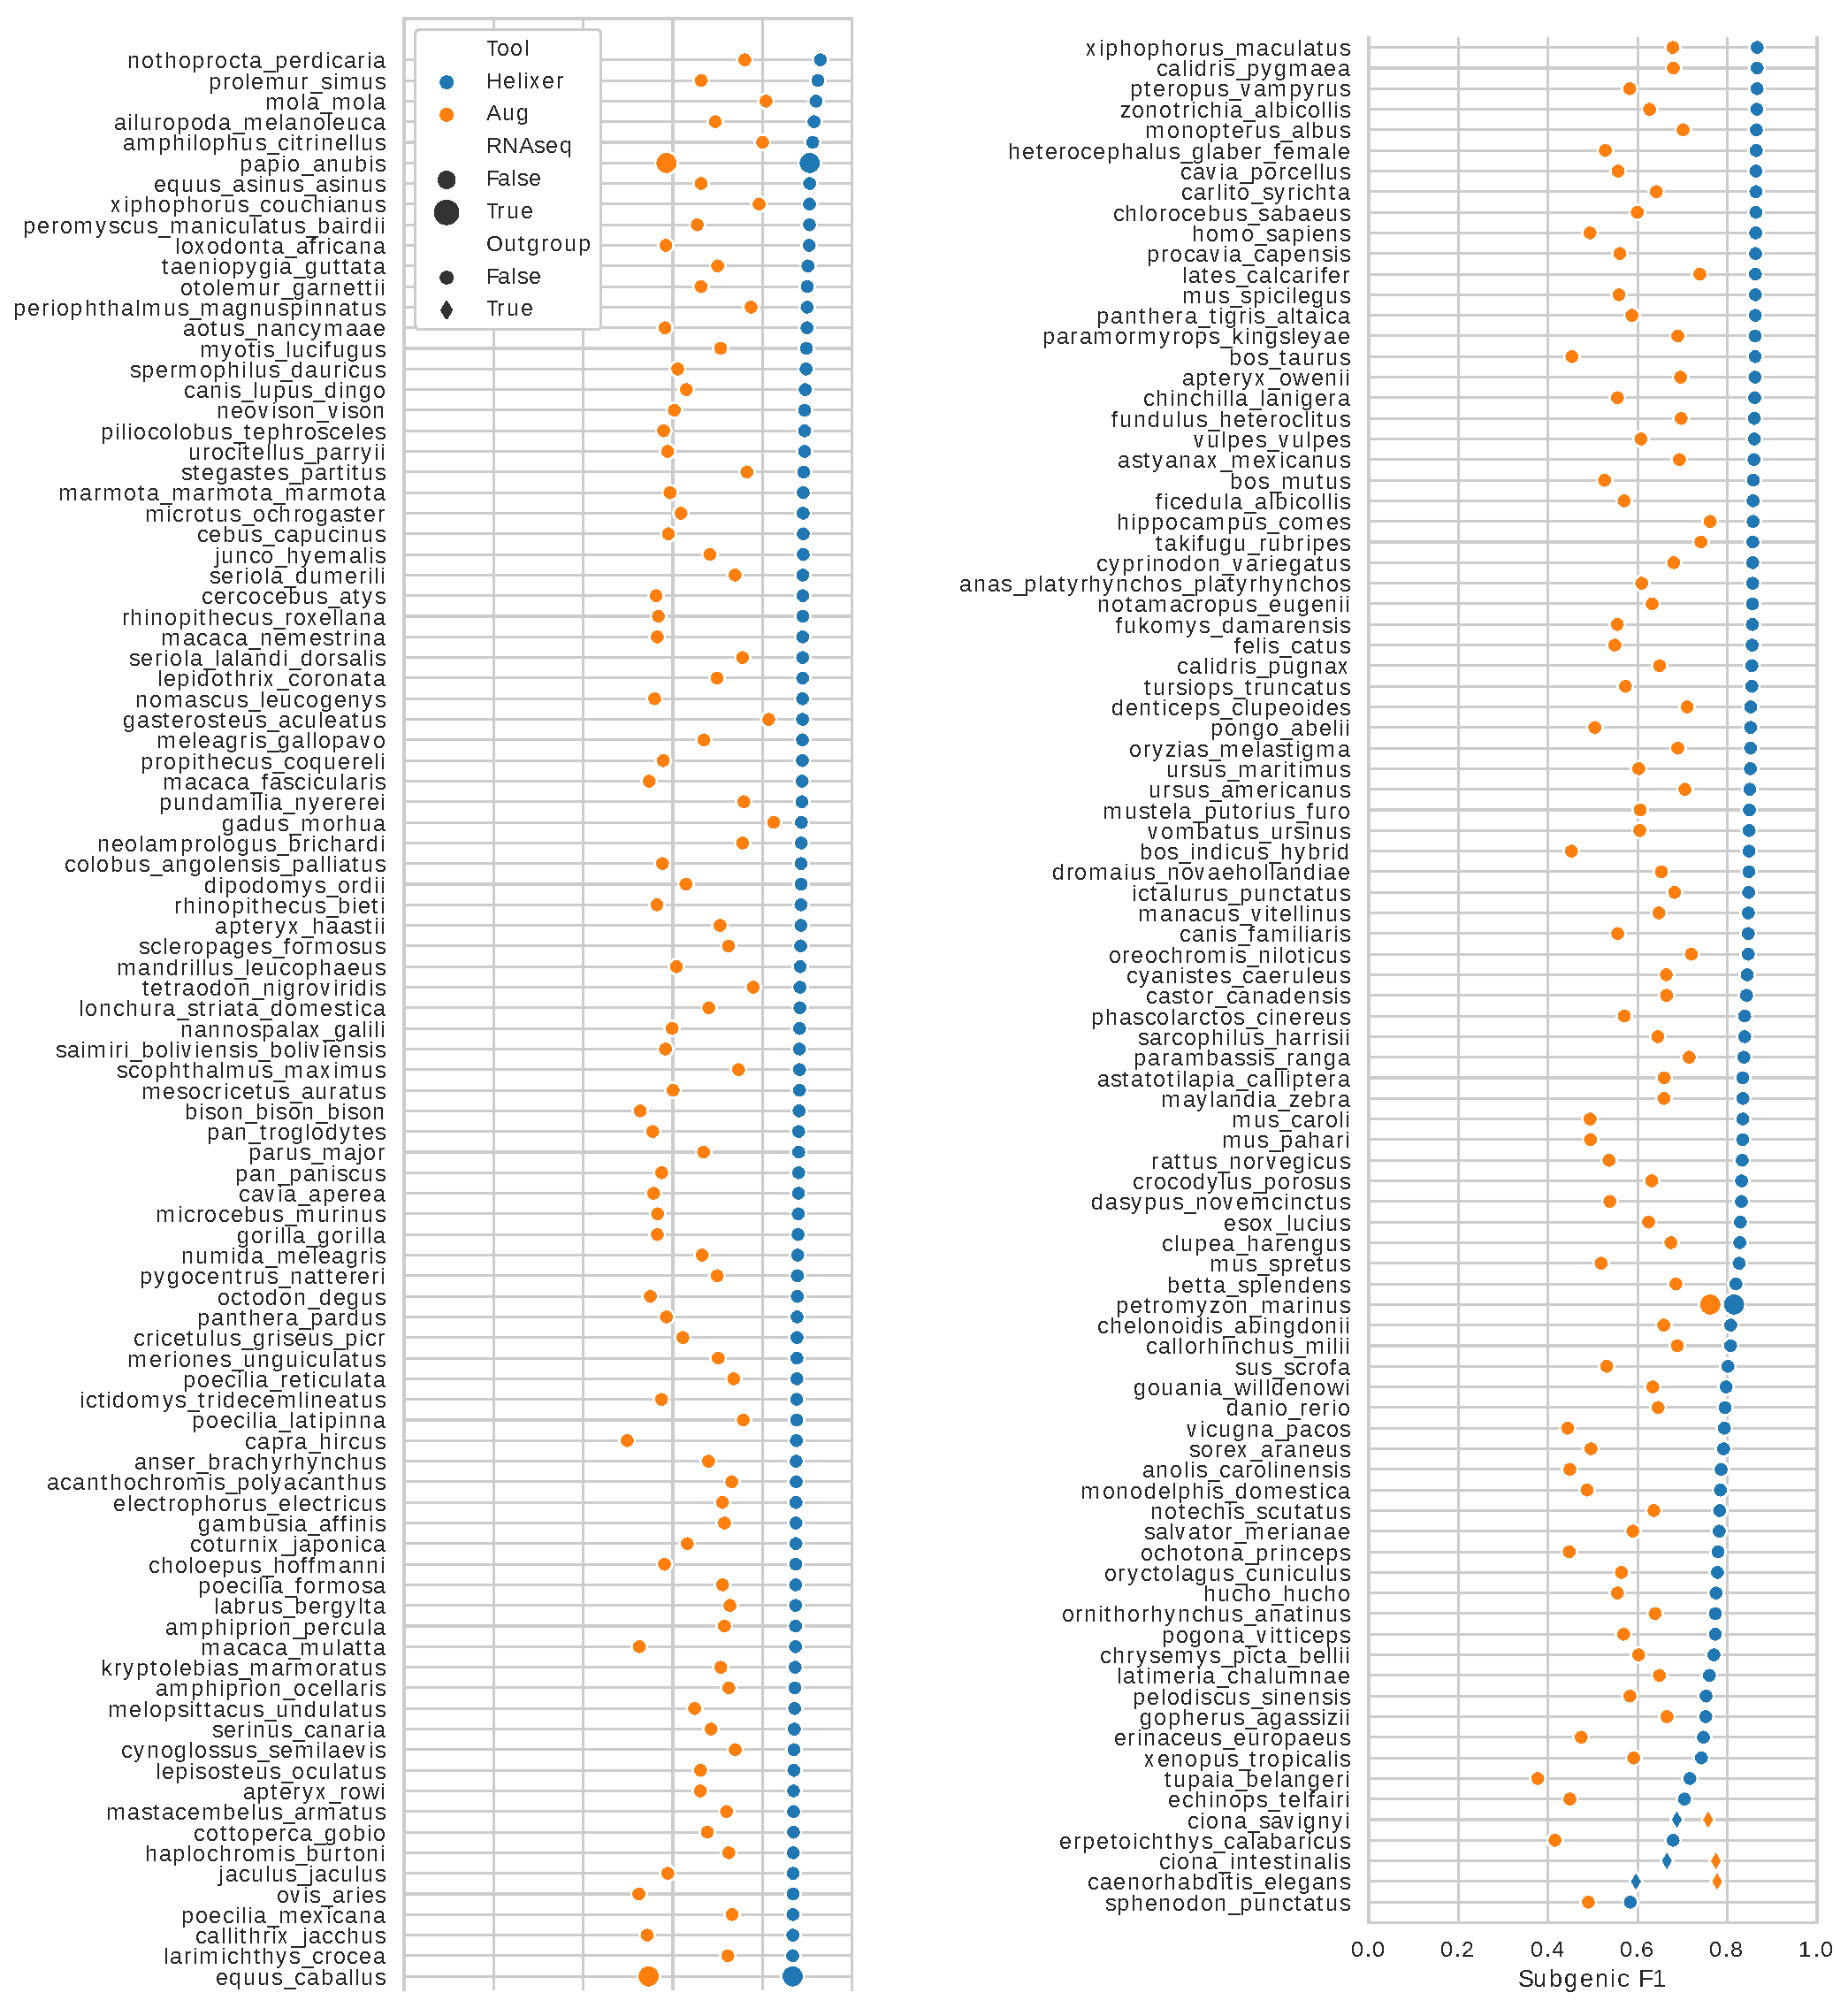
\includegraphics[width=1.0\textwidth]{images/RNAseq_animals_fit}}
\caption{Visualizes how the performance of Helixer (in consideration of Augustus' performance)
was used to select three animal species (larger points) for detailed RNAseq analysis. The 
species were chosen to have good, medium and poor performance; invertebrates (diamonds) were
not considered as the generalizability and recommended use of the Helixer animal model
currently only extends to vertebrates; candidate species were checked for the availibility of
stranded, paired-end RNAseq data and skipped if none was available.}
\end{figure}

\clearpage
\begin{figure}[!hbt]
\label{supfig:rna_select_plants}
\centerline{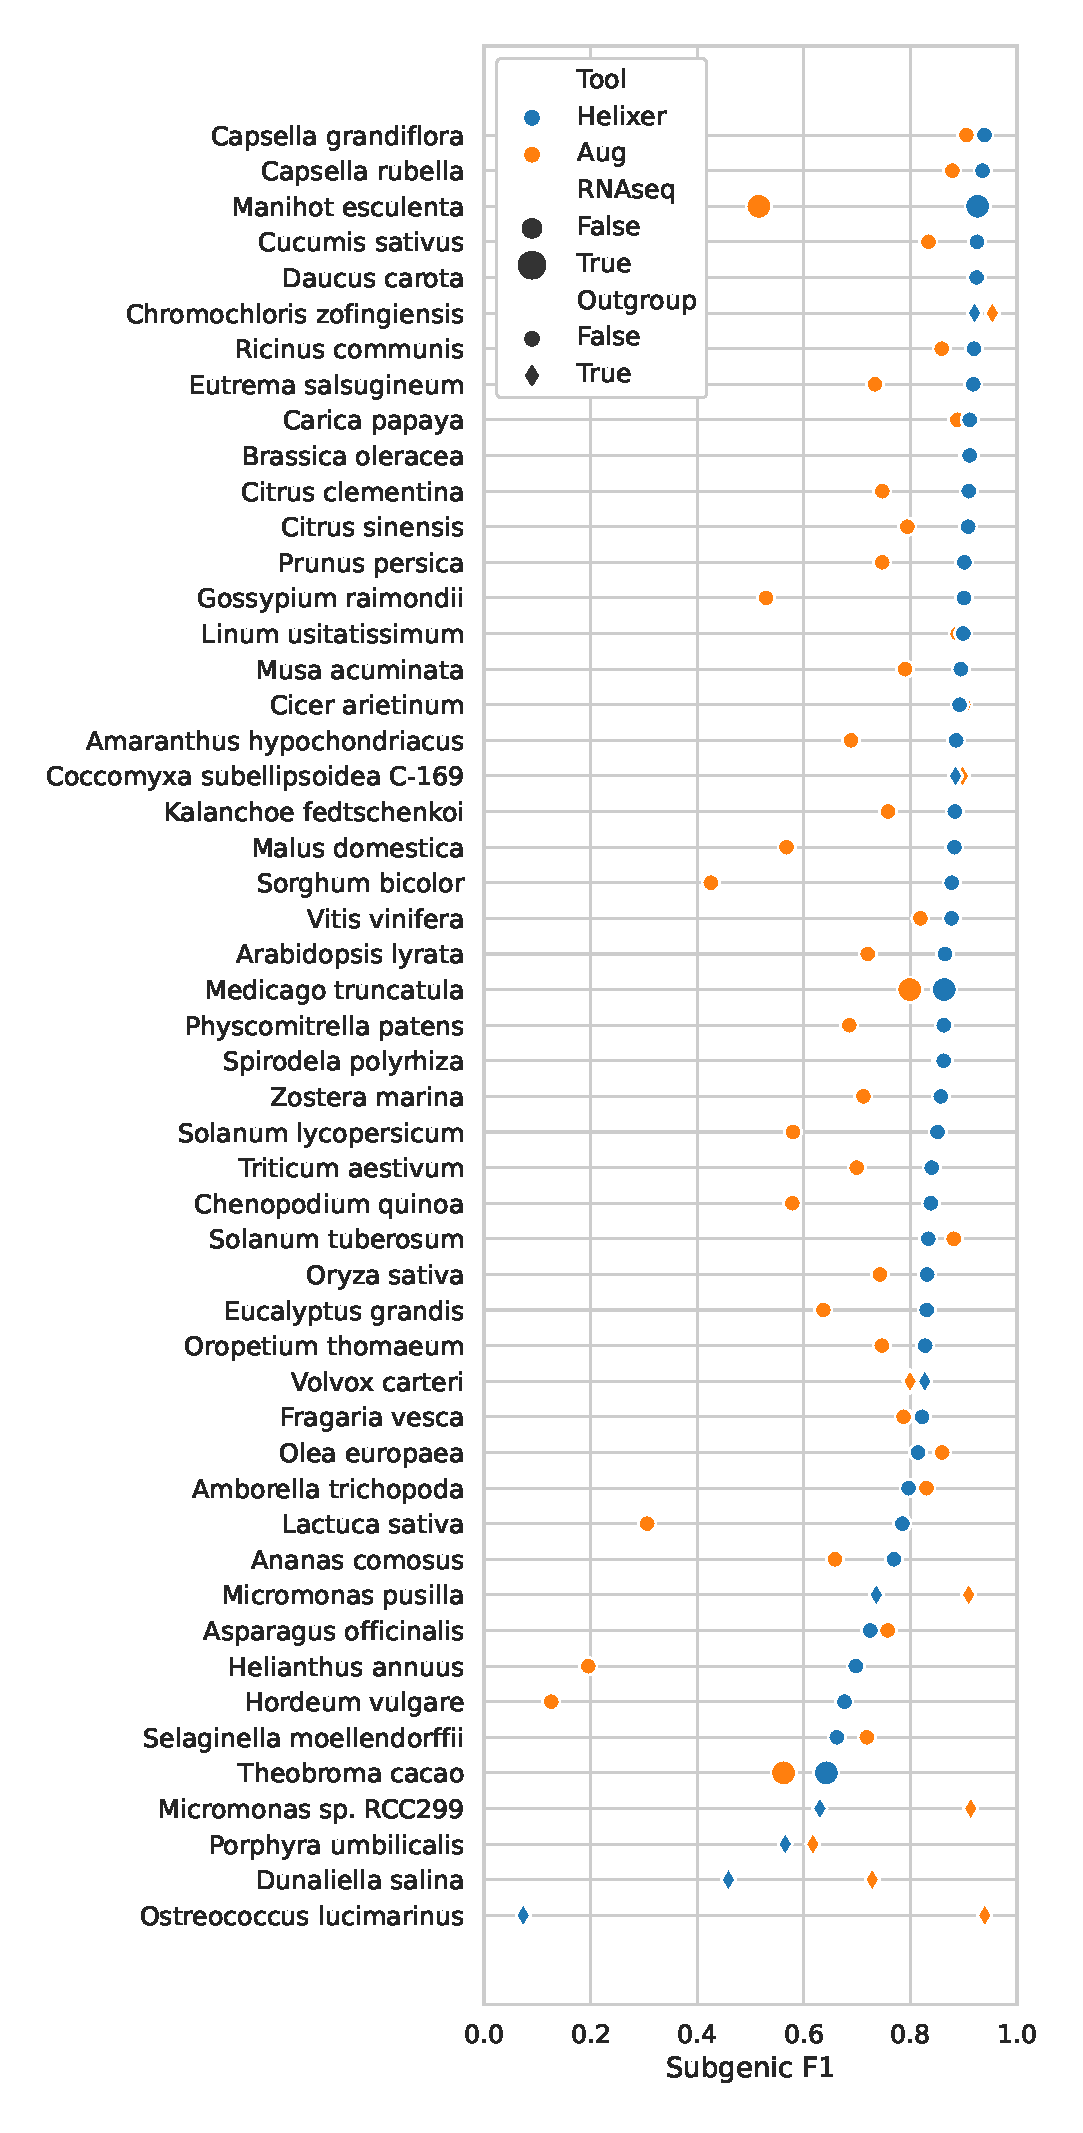
\includegraphics[width=0.5\textwidth]{images/RNAseq_plants}}
\caption{Visualizes how the performance of Helixer (in consideration of Augustus' performance)
was used to select three plant species (larger points) for detailed RNAseq analysis. The 
species were chosen to have good, medium and poor performance; algae (diamonds) were
not considered as the generalizability and recommended use of the Helixer animal model
currently only extends to higher plants; candidate species were checked for the availibility of
stranded, paired-end RNAseq data and skipped if none was available.}
\end{figure}
\clearpage

% RNAseq tested samples table
\begin{table}[!h]
\resizebox{0.8\textwidth}{!}{%
\centering
\begin{tabular}{@{}lll|lll|lll|lll@{}}
\hline
Samples&HQ&S&Samples&HQ&S&Samples&HQ&S&Samples&HQ&S\\
\hline
\\
\textit{P. anubis}\\
\hline
SRS3122053&&&SRS3122094&\checkmark&\checkmark&SRS3270781&&&SRS3270847&&\\
SRS3122057&\checkmark&\checkmark&SRS3122111&&&SRS3270785&&&SRS3270853&&\\
SRS3122063&\checkmark&\checkmark&SRS3270734&&&SRS3270808&&&SRS3270858&&\\
SRS3122070&&&SRS3270735&&&SRS3270811&&&SRS3270862&&\\
SRS3122074&&&SRS3270737&&&SRS3270812&&&SRS3270863&&\\
SRS3122079&\checkmark&\checkmark&SRS3270738&&&SRS3270821&&&SRS3270870&&\\
SRS3122081&&&SRS3270746&&&SRS3270824&&&SRS3270872&&\\
SRS3122088&&&SRS3270751&&&SRS3270839&&&SRS3270880&&\\
SRS3122092&\checkmark&\checkmark&SRS3270763&&&SRS3270840&&&SRS819311&\checkmark&\checkmark\\
SRS3122093&&&SRS3270773&&&SRS3270841&&&SRS819317&\checkmark&\checkmark\\
\hline
\\
\textit{E. caballus}\\
\hline
ERS1517592&&&ERS2382444&&&ERS2681771&&&SRS2552997&\checkmark&\checkmark\\
ERS1517600&&&ERS2681720&\checkmark&\checkmark&ERS2681772&\checkmark&\checkmark&SRS2553004&\checkmark&\checkmark\\
ERS1517608&&&ERS2681730&&&ERS2681775&&&SRS2770963&&\\
ERS1517617&&&ERS2681733&&&ERS3563898&&&SRS2770972&&\\
ERS1517625&&&ERS2681734&&&SRS1102326&&&SRS3347177&&\\
ERS1517633&&&ERS2681740&&&SRS1102328&&&SRS3347182&&\\
ERS1517641&&&ERS2681742&&&SRS1102336&&&SRS4826859&&\\
ERS2382439&&&ERS2681750&&&SRS2158774&&&SRS4826867&&\\
ERS2382440&&&ERS2681754&&&SRS2158777&&&SRS4890460&\checkmark&\checkmark\\
ERS2382442&&&ERS2681758&&&SRS2158788&&&SRS5330332&\checkmark&\checkmark\\
ERS2382443&&&ERS2681770&&&SRS2552988&\checkmark&\checkmark&SRS5330340&&\\
\hline
\\
\textit{P. marinus}\\
\hline
SRS5315360&\checkmark&\checkmark&SRS5315363&\checkmark&&SRS5315366&\checkmark&&SRS5315369&\checkmark&\\
SRS5315361&\checkmark&\checkmark&SRS5315364&\checkmark&\checkmark&SRS5315367&\checkmark&\checkmark&&&\\
SRS5315362&\checkmark&\checkmark&SRS5315365&\checkmark&\checkmark&SRS5315368&\checkmark&\checkmark&&&\\
\hline
\\
\textit{M. esculenta}\\
\hline
SRS1608507&&&SRS1610089&\checkmark&\checkmark&SRS1610201&&&SRS946172&&\\
SRS1608510&\checkmark&\checkmark&SRS1610128&\checkmark&\checkmark&SRS1610205&\checkmark&\checkmark&SRS946227&&\\
SRS1610036&&&SRS1610150&&&SRS1610207&&&SRS946633&&\\
SRS1610041&&&SRS1610177&&&SRS1610208&&&SRS946650&&\\
SRS1610076&\checkmark&\checkmark&SRS1610181&&&SRS945853&&&SRS946703&&\\
SRS1610079&\checkmark&\checkmark&SRS1610187&&&SRS946078&&&SRS947897&&\\
SRS1610084&\checkmark&\checkmark&SRS1610197&&&SRS946138&&&&&\\
\hline
\\
\textit{M. truncatula}\\
\hline
ERS1556003&&&SRS1948297&&&SRS3700721&\checkmark&&SRS4425365&\checkmark&\\
ERS1556006&&&SRS1948300&&&SRS3700725&\checkmark&\checkmark&SRS4538246&&\\
ERS1556009&&&SRS1948304&\checkmark&&SRS4425341&&&SRS4538249&&\\
ERS1556012&&&SRS1948306&&&SRS4425343&\checkmark&&SRS5045319&&\\
ERS1556015&&&SRS1948309&&&SRS4425346&\checkmark&\checkmark&SRS5045322&&\\
ERS1556018&\checkmark&&SRS1948313&\checkmark&\checkmark&SRS4425347&\checkmark&\checkmark&SRS5045325&&\\
ERS1556021&&&SRS1948315&&&SRS4425350&\checkmark&&SRS5045328&&\\
ERS1556024&&&SRS3700712&\checkmark&&SRS4425353&&&SRS5045330&&\\
SRS1736395&\checkmark&\checkmark&SRS3700715&\checkmark&&SRS4425356&\checkmark&\checkmark&SRS5045334&&\\
SRS1736398&\checkmark&&SRS3700717&&&SRS4425357&&&SRS5045337&&\\
SRS1948293&&&SRS3700718&\checkmark&\checkmark&SRS4425364&\checkmark&&&&\\
\hline
\\
\textit{T. cacao}\\
\hline
SRS5244538&\checkmark&&SRS5244546&\checkmark&\checkmark&SRS5244554&&&SRS5244562&\checkmark&\checkmark\\
SRS5244539&&&SRS5244547&&&SRS5244555&&&SRS5244563&&\\
SRS5244540&&&SRS5244548&&&SRS5244556&\checkmark&\checkmark&SRS5244564&&\\
SRS5244541&&&SRS5244549&&&SRS5244557&\checkmark&&SRS5244565&\checkmark&\checkmark\\
SRS5244542&&&SRS5244550&&&SRS5244558&&&SRS5244566&&\\
SRS5244543&\checkmark&\checkmark&SRS5244551&&&SRS5244559&&&SRS5244567&&\\
SRS5244544&\checkmark&\checkmark&SRS5244552&&&SRS5244560&&&SRS5244568&&\\
SRS5244545&&&SRS5244553&\checkmark&\checkmark&SRS5244561&&&&&\\
\hline
\end{tabular}}
\caption{List of RNAseq samples that were selected for processing, whether they were of high quality (HQ), and 
finally, whether they were ultimately selected (S) for merging and use in coverage calculation.}
\label{suptab:rnaseq_samples}
\end{table}
\clearpage
%


\newpage
\section{Longer Sequence Input}
\label{sec:longer}
\begin{table}[!h]
%\renewcommand\thetable{S5}
\centering
\begin{tabular}{@{}lll@{}}
\hline
Class & Input Length in bp\\ [0.5ex]
\hline
Mammalia & 200.000 \\
Non-avian Reptilia & 200.000 \\
Aves & 100.000 \\
Amphibia & 100.000 \\
Actinopterygii & 50.000 \\
Chondrichthyes & 50.000 \\
Actinistia & 50.000 \\
Ascidiacea & 20.000 \\
Insecta & 20.000 \\
\hline
\end{tabular}
\caption{Input sequence length for each phylogenetic class present in our animal dataset. As a rule of thumb, we found the input length should be proportional to the average gene length of the class while staying in the interval [20.000, 200.000]. If the N75 of a specific species was less than twice as high as the supposed sequence length it was lowered until either this criteria as met or a length of 50.000 was reached. }
\label{suptab:prediction_lengths}
\end{table}

\newpage
\section{Effect of Overlapping by Species}
\label{sec:overlapping}

The following plots show the effect of overlapping for each species we worked with individually. The plots are ordered with descending N75, as we found that overlapping tends to produce less desirable patterns in the prediction quality for the very fragmented genomes. 

\subsection{Animals}
\newpage
\def \overlapscale{1.07}
\begin{figure}[!h]
\centerline{\includegraphics[width=\overlapscale\textwidth]{images/overlapping/montage_animals1}}
\end{figure}
\begin{figure}[!h]
\centerline{\includegraphics[width=\overlapscale\textwidth]{images/overlapping/montage_animals2}}
\end{figure}
\begin{figure}[!h]
\centerline{\includegraphics[width=\overlapscale\textwidth]{images/overlapping/montage_animals3}}
\end{figure}
\begin{figure}[!h]
\centerline{\includegraphics[width=\overlapscale\textwidth]{images/overlapping/montage_animals4}}
\end{figure}
\begin{figure}[!h]
\centerline{\includegraphics[width=\overlapscale\textwidth]{images/overlapping/montage_animals5}}
\end{figure}
\begin{figure}[!h]
\centerline{\includegraphics[width=\overlapscale\textwidth]{images/overlapping/montage_animals6}}
\end{figure}
\begin{figure}[!h]
\centerline{\includegraphics[width=\overlapscale\textwidth]{images/overlapping/montage_animals7}}
\end{figure}
\begin{figure}[!h]
\centerline{\includegraphics[width=\overlapscale\textwidth]{images/overlapping/montage_animals8}}
\end{figure}
\begin{figure}[!h]
\centerline{\includegraphics[width=\overlapscale\textwidth]{images/overlapping/montage_animals9}}
\end{figure}
\begin{figure}[!h]
\centerline{\includegraphics[width=\overlapscale\textwidth]{images/overlapping/montage_animals10}}
\end{figure}
\begin{figure}[!h]
\centerline{\includegraphics[width=\overlapscale\textwidth]{images/overlapping/montage_animals11}}
\end{figure}
\begin{figure}[!h]
\centerline{\includegraphics[width=\overlapscale\textwidth]{images/overlapping/montage_animals12}}
\end{figure}
\begin{figure}[!h]
%\renewcommand\thefigure{S5}
\centerline{\includegraphics[width=1.2\textwidth]{images/overlapping/montage_animals13}}
\caption{Effect of overlapping on the sequence positions wise bias ordered by descending N75 for all animals genomes individually.}
\label{supfig:overlapping_animals}
\end{figure}

\clearpage
\subsection{Plants}

\begin{figure}[!h]
\centerline{\includegraphics[width=\overlapscale\textwidth]{images/overlapping/montage_plants1}}
\end{figure}
\begin{figure}[!h]
\centerline{\includegraphics[width=\overlapscale\textwidth]{images/overlapping/montage_plants2}}
\end{figure}
\begin{figure}[!h]
\centerline{\includegraphics[width=\overlapscale\textwidth]{images/overlapping/montage_plants3}}
\end{figure}
\begin{figure}[!h]
%\renewcommand\thefigure{S6}
\centerline{\includegraphics[width=\overlapscale\textwidth]{images/overlapping/montage_plants4}}
\caption{Effect of overlapping on the sequence positions wise bias ordered by descending N75 for all plant genomes individually.}
\label{supfig:overlapping_plants}
\end{figure}


\clearpage
\section{Training Data statistics}
\label{sec:training_data}
\begin{table}[!h]
%\renewcommand\thetable{S6}
\centering
\begin{tabular}{@{}lll@{}}
\hline
& Animals & Plants\\ [0.5ex]
\hline
Average genome size in Gbp& 2.489 (+- 2.073) & 0.914 (+- 0.934) \\
Average gene length & 25,672 (+- 16,605) & 3,509 (+- 906)\\
Geenuff error rate & 0.253 (+- 0.138) & 0.134 (+- 0.072) \\
Fraction of class Intergenic & 0.752 (+- 0.05) & 0.808 (+- 0.106) \\
Fraction of class UTR & 0.013 (+- 0.011) & 0.033 (+- 0.023) \\
Fraction of class CDS & 0.028 (+- 0.028) & 0.077 (+- 0.052) \\
Fraction of class Intron  & 0.207 (+- 0.023) & 0.083 (+- 0.037) \\
\hline
\end{tabular}
\caption{The description of Table [?] applies here as well.}  % 2
\label{suptab:genome_stats}
\end{table}


\newpage
\section{Dilated CNN Baseline Network Search}
\label{sec:dcnn}
\begin{table}[!h]
%\renewcommand\thetable{S7}
\centering
\begin{tabular}{@{}ll@{}}
\hline
Parameter & Search Space\\ [0.5ex]
\hline
Kernel Size & \{4, 8, 12, 16\}\\
Initial Filter Depth & \{32, 64, 96, 128\}\\
Number of Layers Before Doubling Filter Count & \{1, 2\}\\
Dilation Multiplier & \{2, 3\}\\
Number of Convolutional Layers & \{2, 3, 4, 5, 6, 7, 8\}\\
Number of Hidden Fully Connected (FC) Layers & \{0, 1, 2\}\\	
Dropout Used on FC and Final Conv Layer Output & \{0.0, 0.01, 0.1, 0.2, 0.3\}\\
Learning Rate & \{1e-3, 1e-4\}\\
\hline
\end{tabular}
\caption{Above are all parameters used during neural architecture search for the dilated CNN baseline. The same overall space was used for plant and animal data. We did, however, run multiple distinct searches that sometimes only operated over a subset of the given parameters. This was done as those seemed to be the most promising. We for example restricted the search space of the number of LSTM layers to the highest 3 values in later runs. Decisions were guided by the Genic F1 on the validation set of exactly the same data we trained our final LSTM models with. Runs with a Genic F1 below 0.5 after 10 epochs were stopped and the overall maximum epoch was 15. The performances seemed to be leveling off well before that. The batch size used for almost all runs was 32, the dilation was capped to 81 and the size of each fully connected layer was fixed at 128. New parameters where chosen at random. The implementation and parameter space is very roughly based on \citep{gupta2017dilated} and can be found in the Helixer source code repository. In total, we trained 30 models for the animals and 48 with the plant data.}
\label{suptab:dcnn_xval}
\end{table}

\begin{table}[!h]
%\renewcommand\thetable{S8}
\centering
\begin{tabular}{@{}lll@{}}
\hline
Parameter & Animals & Plants\\ [0.5ex]
\hline
Kernel Size & 16 & 16\\
Initial Filter Depth & 96 & 32\\
Number of Layers Before Doubling Filter Count & 2 & 2\\
Dilation Multiplier & 3 & 3\\
Number of Convolutional Layers & 6 & 8\\
Number of Hidden Fully Connected (FC) Layers & 2 & 0\\
Dropout Used on FC Output & 0.0 & 0.0\\
Learning Rate & 1e-4 & 1e-3\\
\hline
\end{tabular}
\caption{The parameters of the dilated CNN model that performed the best according to the Genic F1 of the validation data of the respective training genomes. The best animal model has circa 4.6 million parameters; the best plant model around 2.1 million.}
\label{suptab:dcnn_params}
\end{table}

\newpage
\section{Evaluation against RNAseq}
\label{sec:rnaseq_eval}


\begin{figure}[!h]
\label{supfig:cov_example_02}

%\renewcommand\thefigure{S7}
\centerline{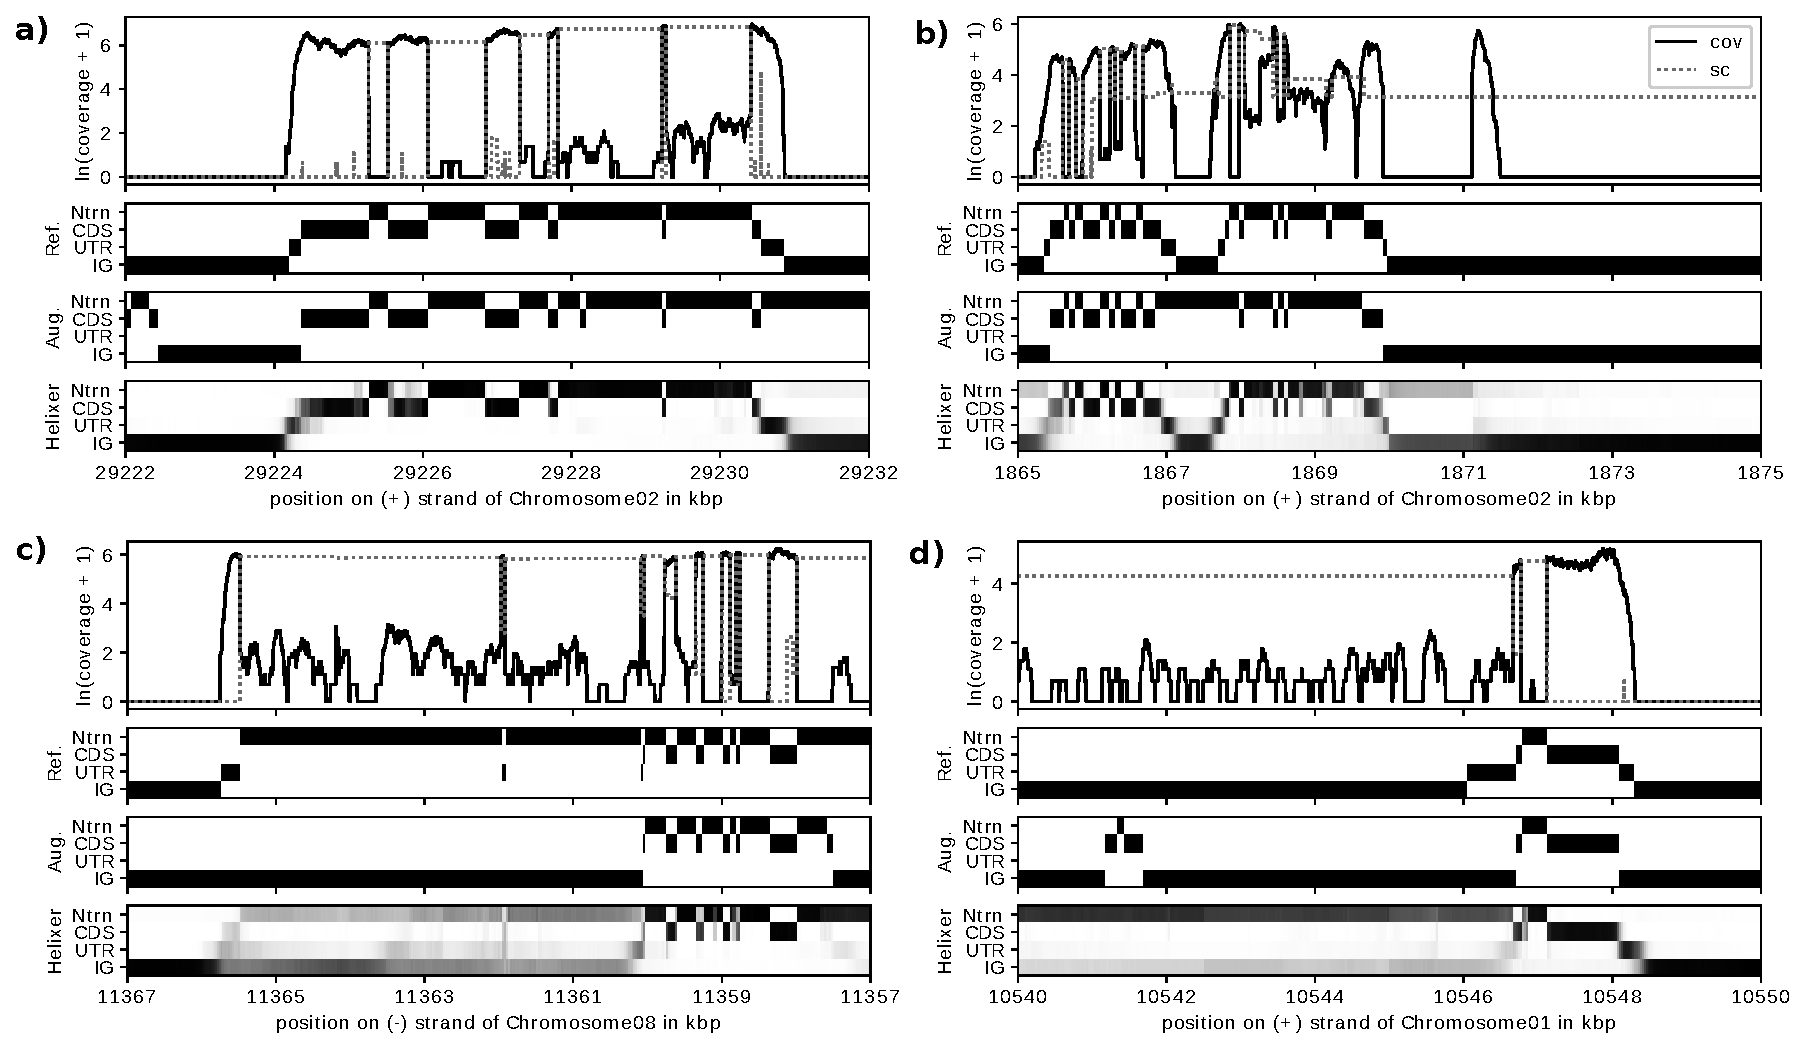
\includegraphics[width=\textwidth]{images/cov_examples/cov_example_002}}
\caption{
Four additional example helixer predictions in the context of RNAseq data, the reference,
and Augustus' prediction for {\it M. esculenta}. The examples were chosen so
that a) Helixer had high accuracy against the reference and the reference
was supported by the RNAseq data, b) Helixer had high accuracy but the
reference was not supported by the RNAseq data, c) Helixer had low accuracy
and the reference was supported by the RNAseq data, and d) helixer had low
accuracy but the reference was not supported by RNAseq data. Plotability was
a major secondary consideration. Each subplot shows from top to
bottom i) the natural log of the coverage (``cov", solid) and spliced coverage
(``sc", dotted) + 1, ii) the reference annotation in matrix form, iii)
Augustus' predictions in matrix form, and iv) Helixer's predictions. The reference
and Augustus have either 0 (white) or 1 (black) for each base pair and category, while
Helixer emits a probability from 0-1 represented via gray-scale. ``Ntrn" stand
for intron, and ``IG" stands for intergenic.
}
\end{figure}

\begin{figure}[!h]
\label{supfig:cov_example_03}
%\renewcommand\thefigure{S8}
\centerline{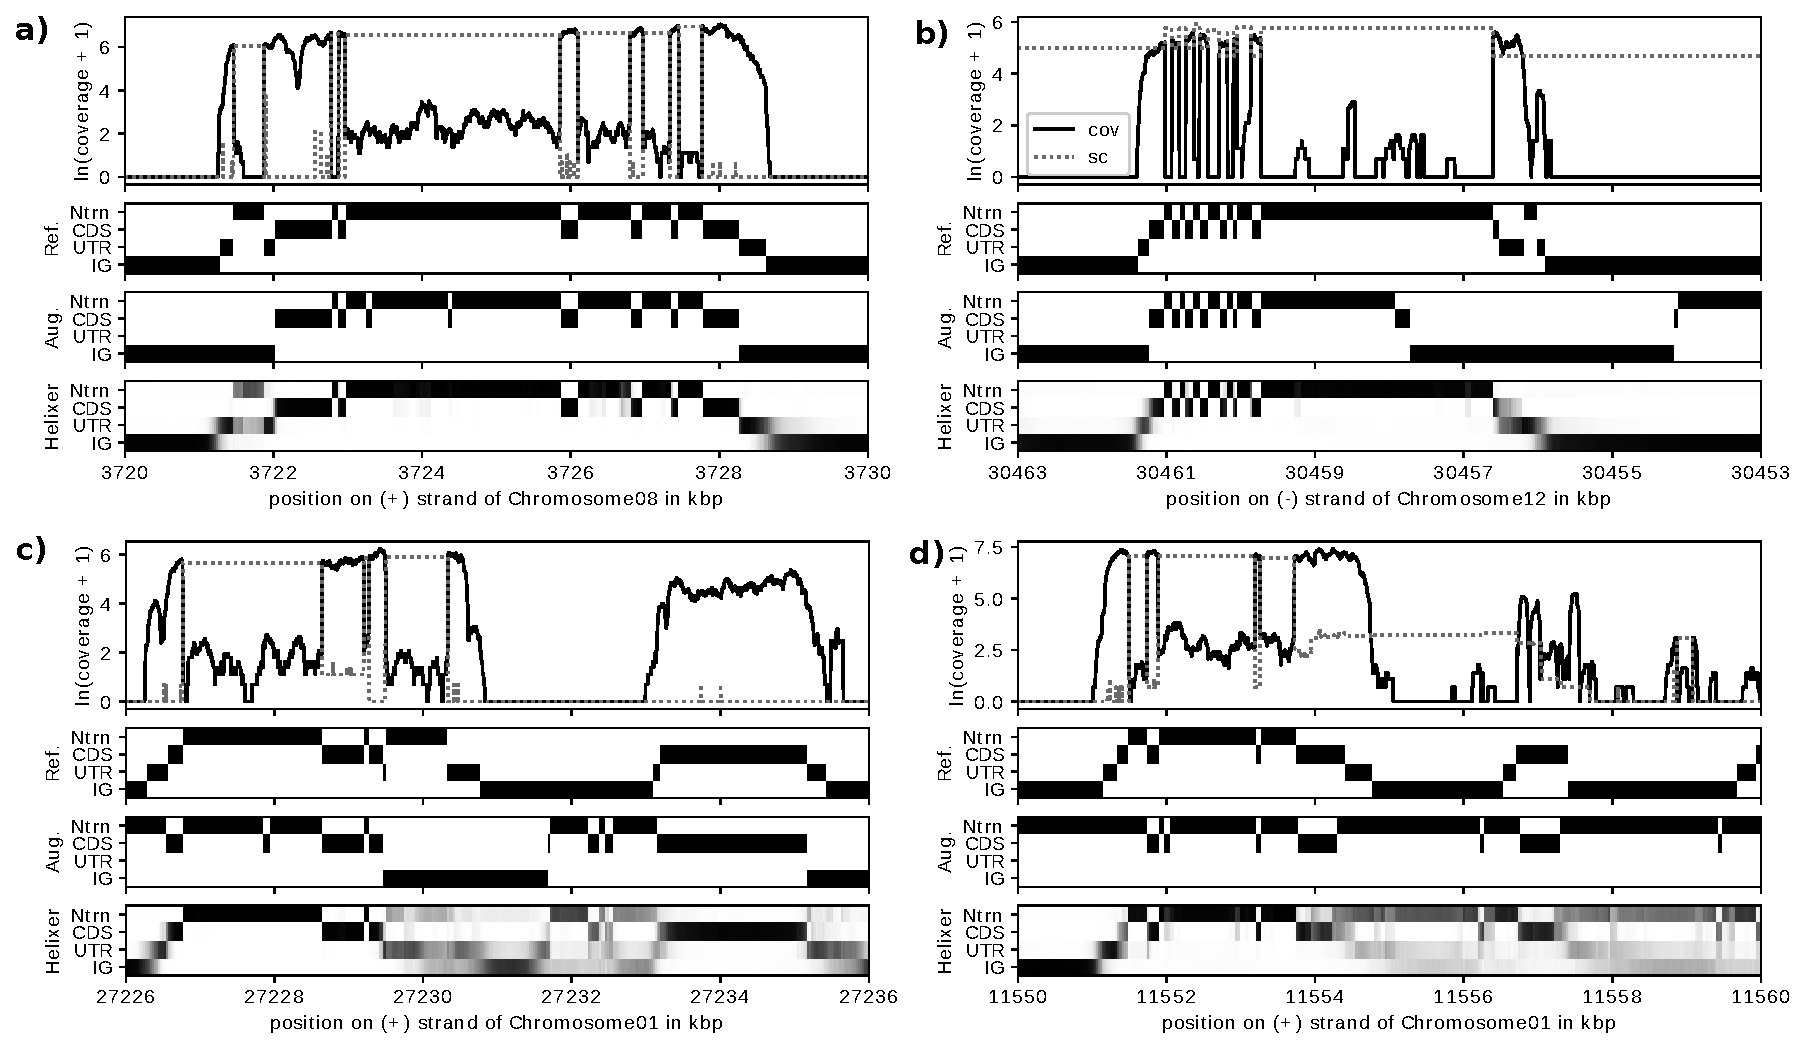
\includegraphics[width=\textwidth]{images/cov_examples/cov_example_003}}
\caption{
Four additional example helixer predictions in the context of RNAseq data, the reference,
and Augustus' prediction for {\it M. esculenta}. The examples were chosen so
that a) Helixer had high accuracy against the reference and the reference
was supported by the RNAseq data, b) Helixer had high accuracy but the
reference was not supported by the RNAseq data, c) Helixer had low accuracy
and the reference was supported by the RNAseq data, and d) helixer had low
accuracy but the reference was not supported by RNAseq data. Plotability was
a major secondary consideration. Each subplot shows from top to
bottom i) the natural log of the coverage (``cov", solid) and spliced coverage
(``sc", dotted) + 1, ii) the reference annotation in matrix form, iii)
Augustus' predictions in matrix form, and iv) Helixer's predictions. The reference
and Augustus have either 0 (white) or 1 (black) for each base pair and category, while
Helixer emits a probability from 0-1 represented via gray-scale. ``Ntrn" stand
for intron, and ``IG" stands for intergenic.
}
\end{figure}

\begin{figure}[!h]
%\renewcommand\thefigure{S9}
\label{supfig:UTRs_animals}
\centerline{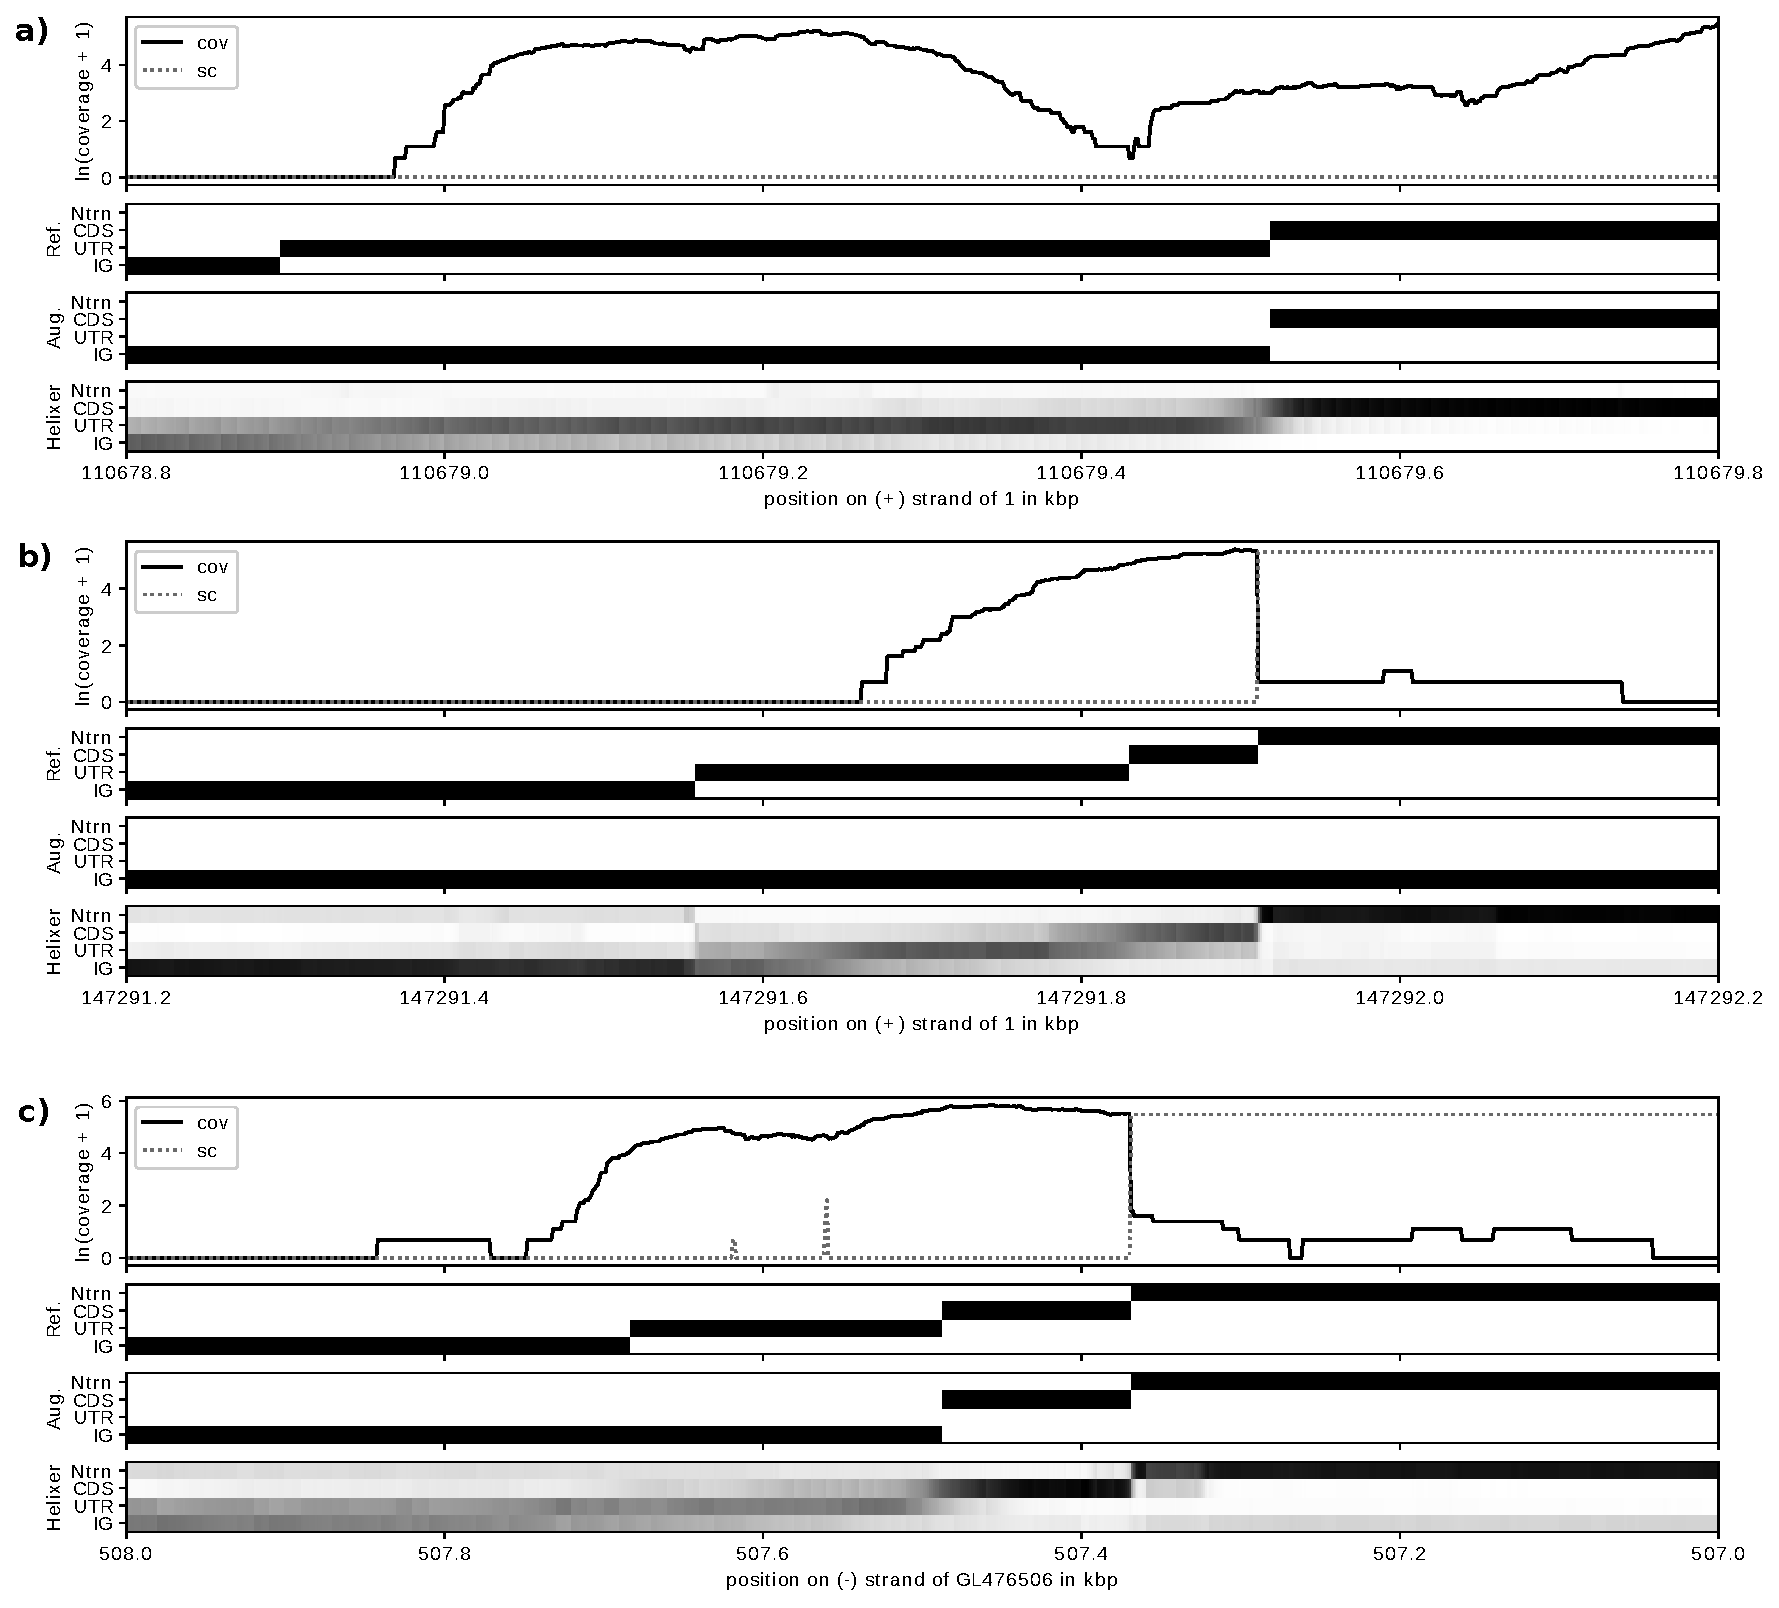
\includegraphics[width=\textwidth]{images/cov_examples/cov_example_UTRs_animals}}
\caption{
One example of helixer's gradual UTR to intergenic transition predictions 
from each RNAseq evaluation animal species in the context of RNAseq data, the reference,
and Augustus' prediction. The species are
a) {\it P. anubis}, b) {\it E. caballus} and c) {\it P. marinus}. Each subplot shows from top to
bottom i) the natural log of the coverage (``cov", solid) and spliced coverage
(``sc", dotted) + 1, ii) the reference annotation in matrix form, iii)
Augustus' predictions in matrix form, and iv) Helixer's predictions. The reference
and Augustus have either 0 (white) or 1 (black) for each base pair and category, while
Helixer emits a probability from 0-1 represented via gray-scale. ``Ntrn" stand
for intron, and ``IG" stands for intergenic.
}
\end{figure}

\begin{figure}[!h]
%\renewcommand\thefigure{S10}
\label{supfig:UTRs_plants}
\centerline{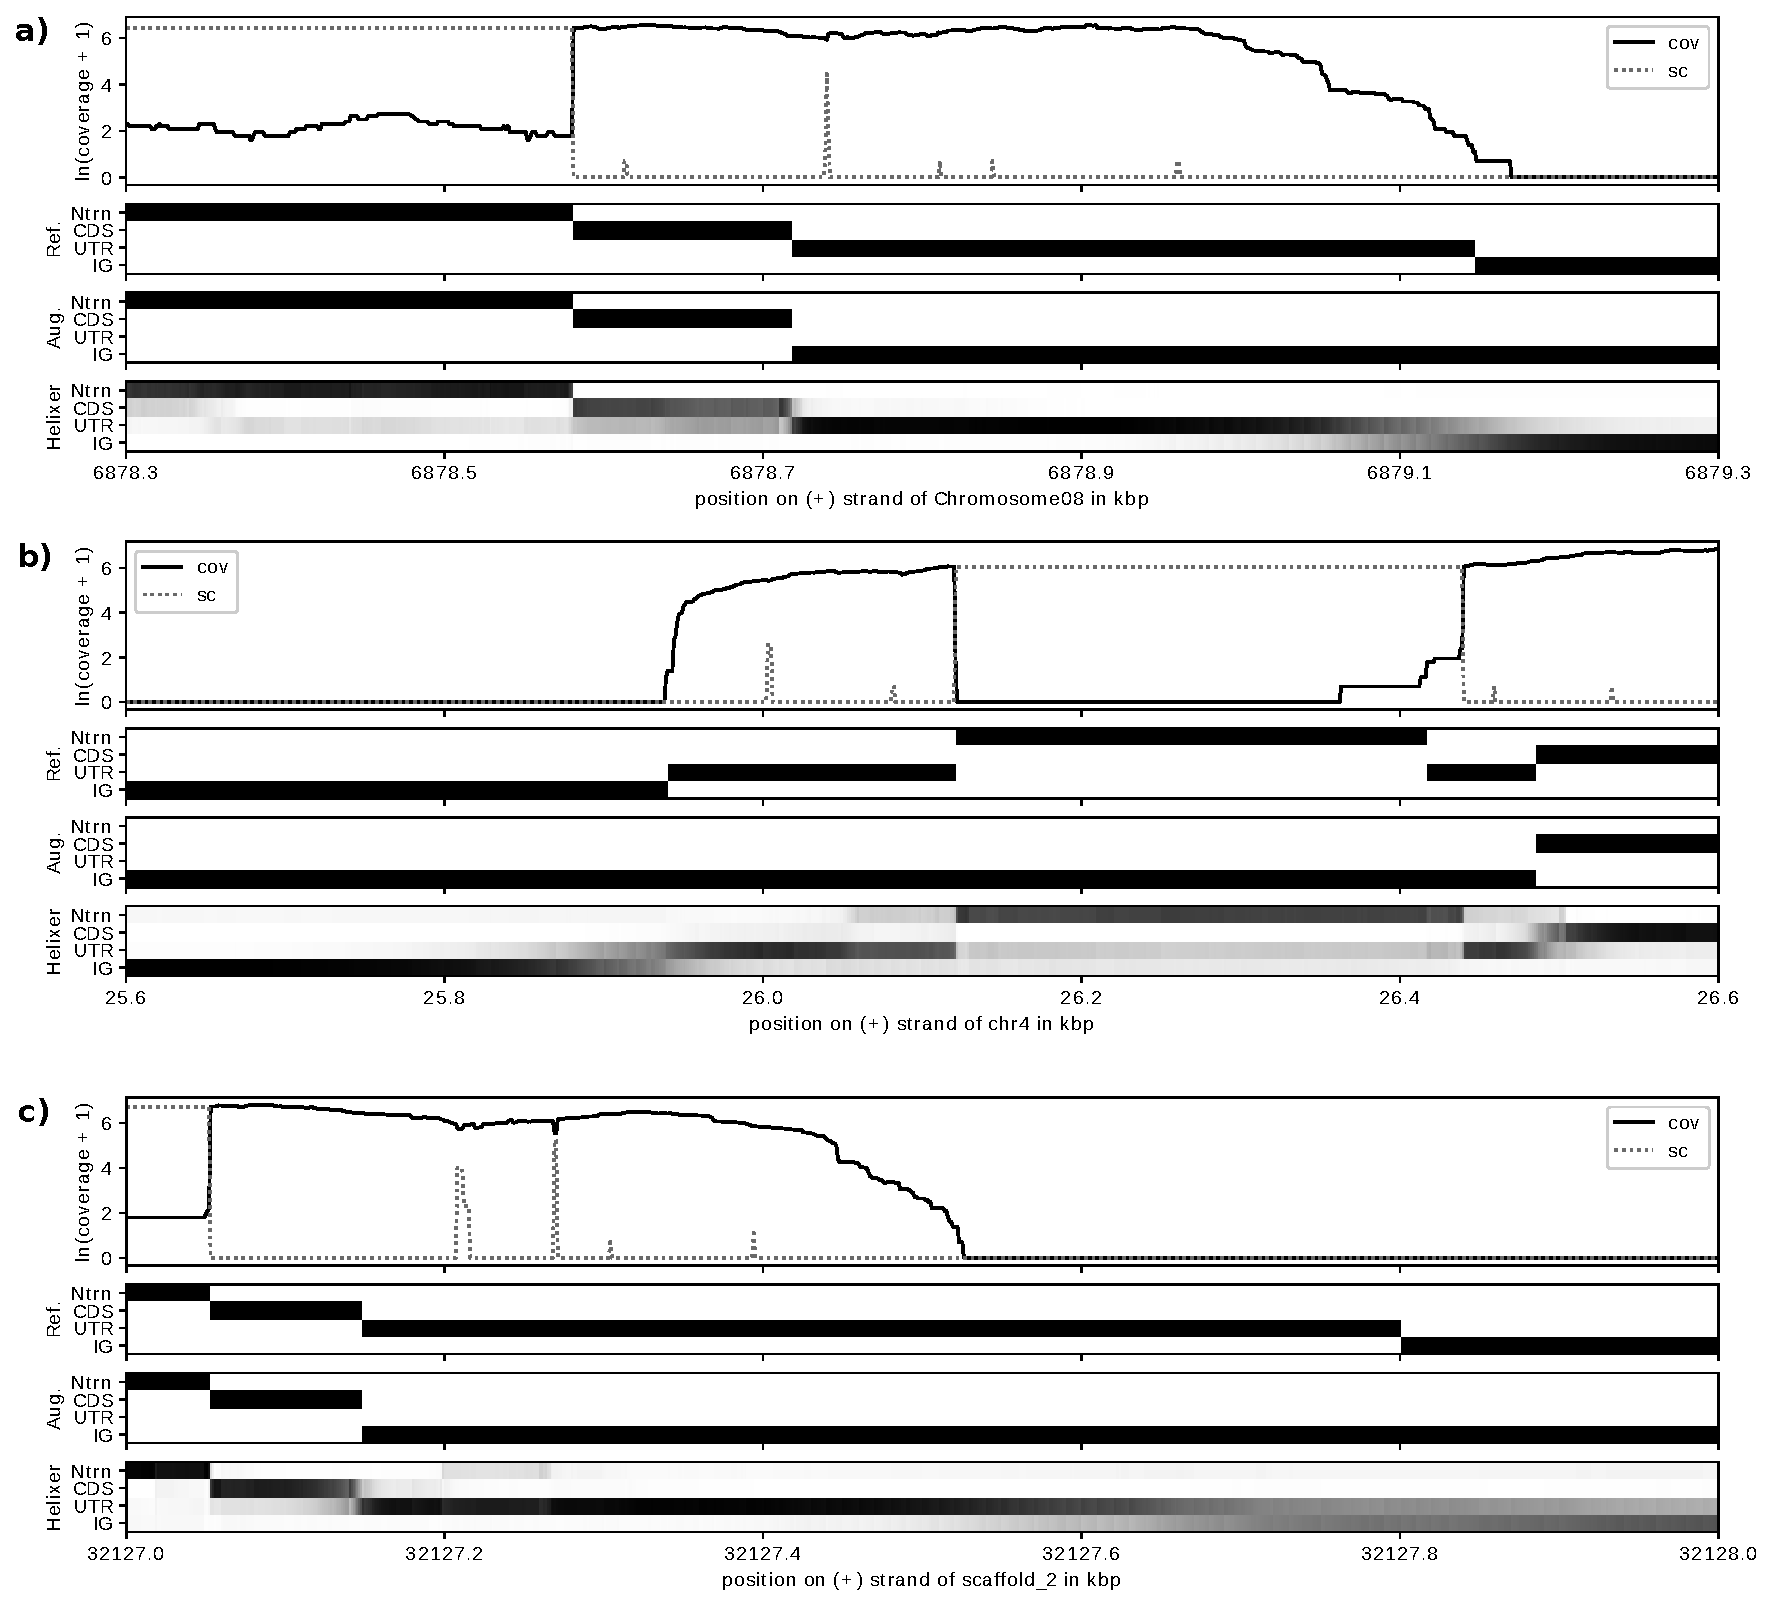
\includegraphics[width=\textwidth]{images/cov_examples/cov_example_UTRs_plants}}
\caption{
One example of helixer's gradual UTR to intergenic transition predictions 
from each RNAseq evaluation plant species in the context of RNAseq data, the reference,
and Augustus' prediction. The species are
a) {\it M. esculenta}, b) {\it M. truncatula} and c) {\it T. cacao}. Each subplot shows from top to
bottom i) the natural log of the coverage (``cov", solid) and spliced coverage
(``sc", dotted) + 1, ii) the reference annotation in matrix form, iii)
Augustus' predictions in matrix form, and iv) Helixer's predictions. The reference
and Augustus have either 0 (white) or 1 (black) for each base pair and category, while
Helixer emits a probability from 0-1 represented via gray-scale. ``Ntrn" stand
for intron, and ``IG" stands for intergenic.
}
\end{figure}


\begin{figure}[!h]
%\renewcommand\thefigure{S11}
\label{supfig:average_vs_ref}
\centerline{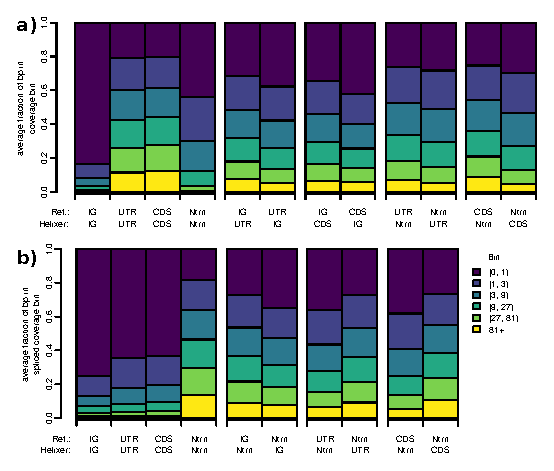
\includegraphics[]{images/cov_examples/average_vs_ref}}
\caption{
Fraction of bp with color-indicated a) coverage and b) spliced coverage of genomic positions
broken down by the confusion matrix of the reference and Helixer's predictions. Categories
are only displayed if they can be meaningfully compared by examining a) coverage or b) spliced
coverage. The displayed fractions are the averages of the individual fractions for the
six RNAseq-evaluation species. The left-most bars show cases where the two tools agree,
while the remaining bars show paired conflicts. ``Ntrn" stand
for intron, and ``IG" stands for intergenic.
}
\end{figure}

\begin{figure}[!h]
%\renewcommand\thefigure{S12}
\label{supfig:each_sp_vs_augustus}
\centerline{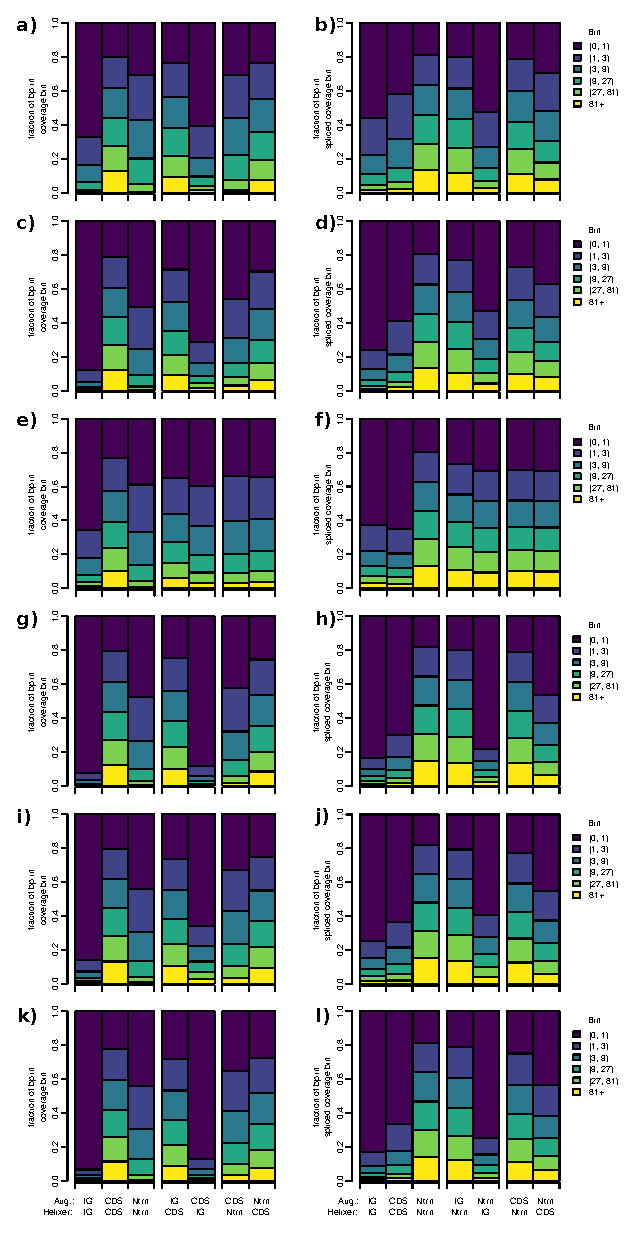
\includegraphics[]{images/cov_examples/each_sp_vs_augustus}}
\caption{
Fraction of bp with color-indicated a, c, e, g, i, k) coverage and b, d, f, h, j, l) spliced coverage of genomic positions
broken down by the confusion matrix of Augustus' and Helixer's predictions. Categories
are only displayed if they can be meaningfully compared by examining coverage or spliced
coverage. The rows show the individual species: a, b) {\it M. esculenta}, c, d) {\it M. truncatula}, 
e, f) {\it T. cacao}, g, h) {\it P. anubis}, i, j) {\it E. caballus} and k, l) {\it P. marinus} . 
The left-most bars show cases where the two tools agree,
while the remaining bars show paired conflicts. ``Ntrn" stand
for intron, and ``IG" stands for intergenic.
}
\end{figure}

\begin{figure}[!h]
%\renewcommand\thefigure{S13}
\label{supfig:each_sp_vs_ref}
\centerline{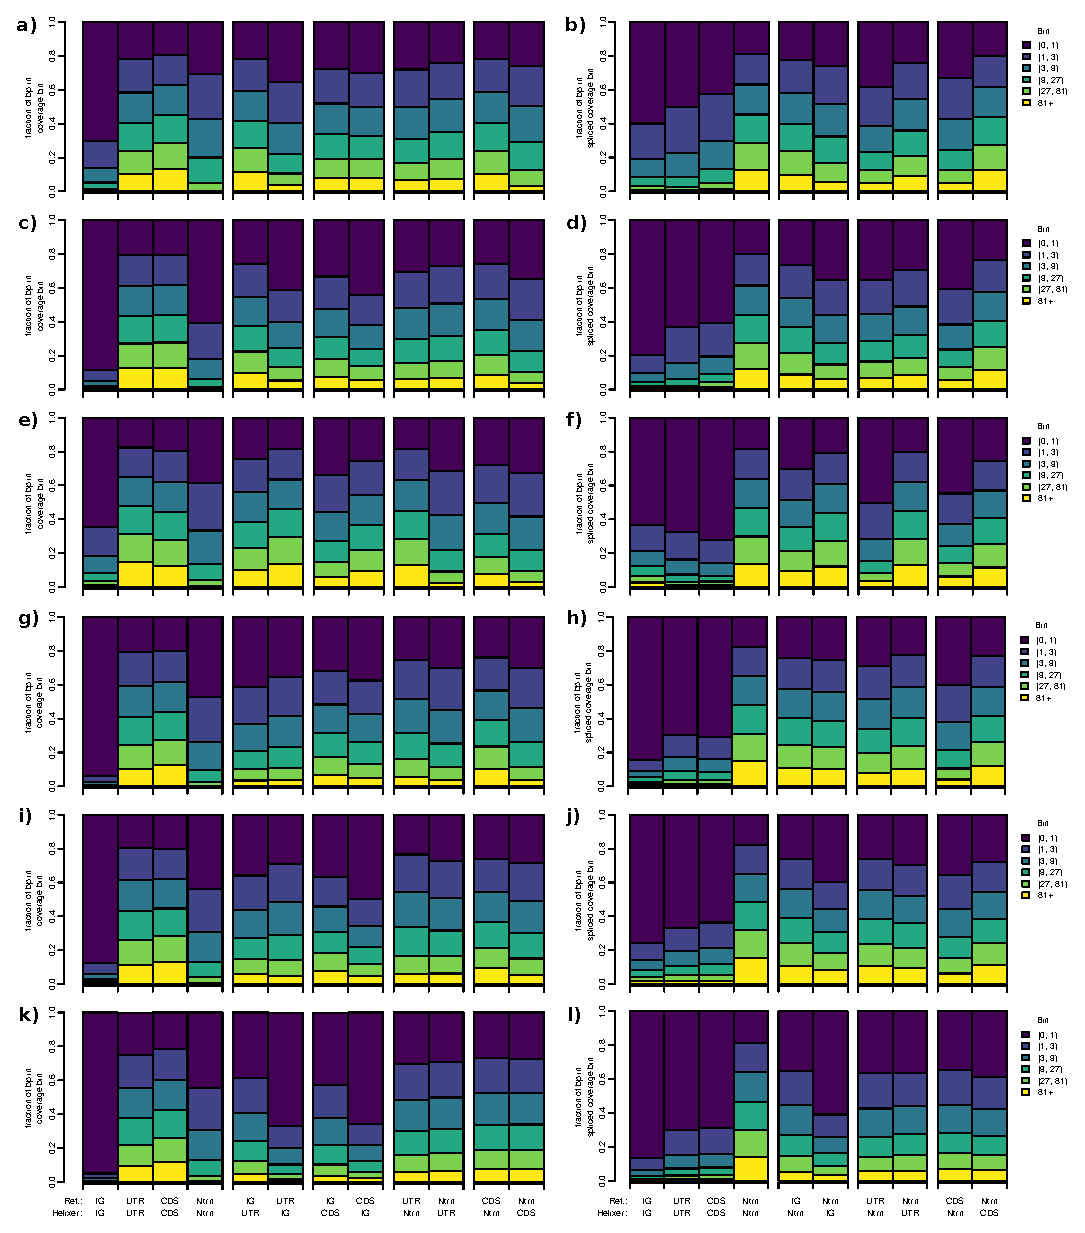
\includegraphics[]{images/cov_examples/each_sp_vs_ref}}
\caption{
Fraction of bp with color-indicated a, c, e, g, i, k) coverage and b, d, f, h, j, l) spliced coverage of genomic positions
broken down by the confusion matrix of the reference and Helixer's predictions. Categories
are only displayed if they can be meaningfully compared by examining coverage or spliced
coverage. The rows show the individual species: a, b) {\it M. esculenta}, c, d) {\it M. truncatula}, 
e, f) {\it T. cacao}, g, h) {\it P. anubis}, i, j) {\it E. caballus} and k, l) {\it P. marinus} . 
The left-most bars show cases where the two tools agree,
while the remaining bars show paired conflicts. ``Ntrn" stand
for intron, and ``IG" stands for intergenic.
}
\end{figure}


\clearpage
\renewcommand\refname{Supplemental References}
\bibliographystyle{natbib}
\bibliography{literature}
\clearpage
\end{document}
